\documentclass[DM,toc]{lsstdoc}

\usepackage{subfig}
\usepackage{fancyvrb}
\usepackage{framed}

\graphicspath{{./figures/}}

\def\A{{\tt A}}
\def\B{{\tt B}}
\def\C{{\tt C}}
\def\D{{\tt D}}
\def\E{{\tt E}}
\def\P{{\tt P}}

\title{Report on Winter 2014 Production: Image Differencing}
\date{\today}
\author{
Andrew Becker, Simon Krughoff, Andrew Connolly
}

\setDocChangeRecord{%
\addtohist{}{2014-05-30}{Initial version.}{A.~Becker}
\addtohist{1}{2017-12-29}{Converted to DMTN-069.}{T.~Jenness}
%\addtohist{2}{yyyy-mm-dd}{Future changes}{Future person}
}

\setDocRef{DMTN-069}
\date{2014-05-30}
\setDocUpstreamLocation{\url{https://github.com/lsst-dm/dmtn-069}}

\setDocAbstract{%
The goals of this Winter 2014 (W14) task are to investigate the
effects of differential chromatic refraction (DCR) on the rate of
false positives in image differences.
}

\begin{document}
\maketitle

\section{Summary}

The goals of this Winter 2014 (W14) task are to investigate the
effects of differential chromatic refraction (DCR) on the rate of
false positives in image differences.  We quantify this using a suite
of image simulations that contain no intrinsic variability, and run
the images through the LSST Data Management image subtraction
pipeline, which includes detection and measurement of false positives
(both positive--going and negative--going) in the differences.  As
demonstrated in a similar analysis in Winter 2013 (W13), we are able
to achieve a false detection rate consistent with random Gaussian
fluctuations in the background in the absence of DCR.

The underlying image simulation software ({\tt phoSim}) and the DM
stack have evolved since our W13 work, {\tt phoSim} from v3.2.2 to
v3.3.2 and DM from v7\_2 to v7\_3.  Accordingly, our first subtask was
to reproduce the results of W13, which involve a suite of 15s
$i$--band images taken at a zenith angle of $20.2^{\circ}$ and in
seeings of 0.6, 0.88, and 1.2 arcseconds.  These were differenced
against a 300s $i$--band image generated at the same airmass, with
seeing 0.88''.  The focus of this analysis was the image--vs--template
seeing dependence of the rate of false positives, and how
pre--filtering of the science {\tt Exposures} with their {\tt Psfs}
affects this rate.  We limited our reanalysis to the central sensor of
central raft {\tt 2,2}, and quantitatively (but not exactly) recover
the results of W13.  The second subtask involved the generation of
$g$--band and $r$--band images in the same observing configuration, to
verify there is no wavelength dependence to our results.  We find that
our results are quantitatively similar to those of the first subtask.
We do not see substantial issues with DCR in these data, as expected.

Our third subtask involved creating a similar suite of $gri$--band
images, but at 5 airmasses throughout a single night, using a star
catalog with 3 discrete SEDs.  The data include 2 observations before
meridian crossing at airmasses 1.55 and 1.16, one observation near
zenith, and then 2 observations after the meridian crossing at
airmasses 1.16 and 1.55.  Observations at the same airmass, but before
and after meridian crossing, have different parallactic angles, and
thus different directions of DCR.  This directly tested whether or not
the parallactic angle needs to be a consideration when designing
templates for image subtraction during LSST operations.  We
differenced each of 5 per--airmass templates against each of the 15
science images (binned 5 in airmass and 3 in seeing), and did this in
each of the 3 passbands.  We find that the difference images where the
parallactic angles are aligned yield false positives consistent with
the rates seen above, at all airmasses.  However, when differencing
images taken at one parallactic angle with a template taken at
another, we find a significantly enhanced rate of false positives.
This rate is both passband and seeing dependent, in the sense that the
false positives are more enhanced in the $g$--band than in the
$i$--band, and higher in the better seeing data than in the worse
seeing data.  We find that DCR offsets of 3--6 mas are sufficient to
yield 1\% likelihood of yielding a dipole for the SEDs used, at a
fiducial seeing of 0.6''.  At seeing of 0.88'', offsets of 5--9 mas
yield the same likelihood.  This indicates a narrow range of science
data that zenith templates may be applied to: airmass $<1.05$ for
$r$--band and $<1.15$ for $i$--band.  At airmass 1.25, the interaction
of airmass and orientation difference sets a range of tolerance for a
given relative DCR offset.  At the same airmass, the stars used in the
simulations show a 1\% chance of showing DCR dipoles at orientation
differences of $5^{\circ}, 15^{\circ}, 25^{\circ}$ in $g,r,i$, and in
the same orientation at airmass differences of $0.05, 0.1, 0.15$,
respectively.  This rate should to be examined using a realistic
distribution of SEDs to understand the wider implications of this
study.  In the $g$ (and especially $u$) bands, nearly all examined
combinations of airmass and orientation differences should yield
significant numbers of false positives.  A fourth subtask -- using a
more realistic mixture of stars and galaxies in the input catalog --
was deferred to later analysis, as this is not central to resolving
the DCR issue.

We validated that the amplitudes and orientations of DCR ``dipoles''
are similar both to theory and to the effects designed into the
simulations.  We also find that joint--Psf dipole measurements of
DiaSources tend to overestimate the amplitude of the effect, with a
dependence on seeing.  Finally, we provide extensive documentation on
the generation and data reduction of image simulations, how to design
DCR into the data, and how to interpret the results.

\section{Production Scope and Goals}

The primary goal of this W14 production was to investigate the effects
of DCR on the image differencing process, with the expectation that
this informs the requirements on image differencing templates.  The
current DM baseline is that LSST will have up to 9 templates per
passband per region of sky, binned 3x3 in airmass and seeing.  The
airmass bins are currently segmented only on the zenith distance of
the observation.  However, this design does not account for the angle
that refraction displaces objects within the image, which will be
different for every observation, and which ideally requires a
per--image (in orientation) and per--object (in amplitude) correction
to properly compensate for it.

To examine these effects, we designed a staged analysis where each
successive stage builds on the results of the previous stage, but adds
an additional layer of complexity.  Starting with the base input
catalog and simulation configuration used in the previous W13
analysis, our second subtask included multi--passband sims, while the
third subtask additionally included multi--airmass and
multi--parallactic angle sims.  This final stage was sufficient to
characterizes the effects of DCR on the false positive rate.
Technical details on each of the subtasks are provided in
Appendix~\ref{appx:tasks}.

We generated images in three passbands corresponding to the LSST
$g$--band, $r$--band, and $i$--band filters.  Fifteen--second
``snaps'' were generated at 3 discrete seeings: 0.6'', 0.88'', 1.2''.
One accompanying image subtraction template was also generated (as
opposed to assembled via coaddition) with an effective 300 second
exposure time and a seeing of 0.88''.  All 4 sets of images were
generated for each airmass--filter combination.

After generation we ran the simulated {\tt eImages} through single
frame measurement (SFM) using the script {\tt processEimage.py}.  Note
that we did {\it not} use the raw per--amplifier simulated images,
instead choosing to operate on the {\tt eImages} because the former
would have required the generation of calibration products and
instrument signature removal (ISR).  Had we run in this mode, SFM
would have proceeded using the script {\tt processCcd.py}.

We next ran the images through image differencing, using the 300s
image as the image subtraction template.  For this reason, the derived
class {\tt Winter2013ImageDifferenceTask} (so--called as it was
initially designed for the W13 production cycle) was used, as this
includes a specific flag to use a visit as the template, instead of an
extraction from the coadd repository.  Two sets of image differencing
runs were performed, the first being a ``classical'' analysis and the
second pre--filtering the science image with its Psf\footnote{Briefly,
  the science image is convolved with its Psf, yielding a maximum
  likelihood image for point source detection.  The template is then
  ``Psf''--matched to this image, where Psf is in quotes because the
  signal being matched to is not truly a point spread function.  For
  more details please see:
  \url{https://dev.lsstcorp.org/cgit/LSST/DMS/report/W13report.git}}.
We next ran detection and measurement on each difference image to
extract the {\tt DiaSources} from the images.  We looked at detections
of both positive and negative polarity, and at a detection threshold
of 5--sigma.  Dipoles were identified and measured, and their
separation and orientation compared to what was expected from theory,
and what was expected based on the inputs to {\tt phoSim}.  The
numbers of false positives were recorded as a function of filter,
image seeing, image airmass, and (where applicable) template airmass.
In the following, we reference the 3 bins in seeing as {\tt Seeings
  1,2,3} for seeing = 0.6'', 0.88'', 1.2'', respectively, and the 5
visits at different airmasses as {\tt Visits A,B,C,D,E}.  We briefly
summarize each of the subtasks below.

\subsection{Subtask 1: Reproduce W13 Results Using Current PhoSim}

To ensure that the results of W14 may be compared to the results from
W13, we first validated that the {\tt phoSim} software and DM stack
(and their interaction) had not significantly changed in the interim.
We note that W13 used {\tt phoSim} version v3.2.2 and DM stack v7\_2;
W14 uses v3.3.2 and v7\_3, respectively.  Starting with the W13 {\tt
  phoSim} configuration, we produced simulated images at a single
airmass (1.07) and in a single passband ($i$).  Science images were
simulated at each of the 3 seeing values described above, plus an
image subtraction template image.  We simulated images only for the
central sensor {\tt 1,1} of the central raft {\tt 2,2}.  We performed
image differencing, source detection and measurement, and validated
that the average numbers of false positives were consistent with the
results of W13.  We also analyzed the actual W13 data using the
current version of the DM pipeline, and validated that the total
numbers of false positives were similar to the W13 analysis, with
minor differences.  Results of these analyses are described in
Section~\ref{sec:task1} below.

The {\tt phoSim} configuration files for this subtask are contained in
subdirectory {\tt sims3/} of this repository.  Work on this subtask
resulted in Ticket \#3143, described in Appendix~\ref{sec:3143} below.

\subsection{Subtask 2: Simulate Starfield using Multiple SEDs at a Single Airmass}

Starting with the input trim files to subtask 1 above, we replaced the
SEDs used for the starfield with 3 discrete SEDs chosen to span a
range in color.  We chose a {\tt G0V} star to be our reference source,
and replaced 80\% of the source SEDs with those of SED {\tt
  km20\_6000.fits\_g30\_6020.gz}.  When performing the image
differencing, {\it only} these objects were used for the creation of
the Psf--matching kernel.  This effectively made this set of sources
the reference for the differential refraction.  We then replaced 10\%
of the SEDs with those of a ``blue'' source -- spectrum {\tt
  kp01\_9750.fits\_g45\_9830.gz} representing an {\tt A0V} star -- and
10\% of the SEDs with those of a ``red'' source -- spectrum {\tt
  m2.0Full.dat.gz} representing an {\tt M2.0V} star.  We modified the
brightnesses of the sources in the $i$--band trim file to have
approximately the same S/N as the original sources, given the color of
each star.  We then re--ran the image differencing analysis, and
validated that we were able to difference the $i$--band data to a
similar quality as in subtask 1 above.  The {\tt phoSim} configuration
files for this are contained in subdirectory {\tt sims5/} of this
repository.

We further generated sets of simulations in the $g$--band and
$r$--band using the exact same set of trim files except for the
requested {\tt Opsim\_filter}.  Analysis of these images showed no
color--dependence to our results.  However, because we did not modify
the input brightness distributions for the stars to have similar S/N
in each passband, the results are somewhat compromised due to the
different signal--to--noise distributions.  However, we have not seen
S/N dependence in prior analyses, so do not expect this to
substantially modify our conclusions.  Results of these analyses are
described in Section~\ref{sec:task2} below.  The {\tt phoSim}
configuration files for this are contained in subdirectory {\tt
  sims5gr/} of this repository.

Work on this subtask resulted in Ticket \#3128, described in
Appendix~\ref{sec:3143} below.

\subsection{Subtask 3: Simulate Starfield using Multiple SEDs at Multiple Airmasses}

\begin{table}
\centering
\begin{tabular}{cccccc}
\hline
\multicolumn{6}{|c|}{Subtask 3: PhoSim Visit Configuration} \\ \hline \\
Visit & MJD           & rotSkyPos   & rotTelPos   & Altitude & Airmass \\
\hline
\A    & 51130.111719  & 251.0689567 & 145.7139810 & 40.1     & 1.55 \\
\B    & 51130.176302  & 251.0689567 & 152.2708405 & 59.9     & 1.16 \\
\C    & 51130.272830  & 251.0689567 & 341.0975816 & 89.9     & 1.00 \\
\D    & 51130.272830  & 251.0689567 & 349.8619334 & 59.9     & 1.16 \\
\E    & 51130.433247  & 251.0689567 & 356.4181128 & 40.1     & 1.55 \\
\end{tabular}
\caption[So I can have 2 paragraphs]{Summary of the configuration
  parameters that define each subtask 3 visit \A\B\C\D\E.
  Observations were designed to follow a single star field through
  zenith on a single night, and observed twice before and twice after
  crossing the meridian, as well as at zenith.  Each visit was
  simulated using the same random seed (153555399), in 3 filters ($g$,
  $r$, $i$), and under 4 observing conditions.  These correspond to
  the template image ({\tt Opsim\_rawseeing} = 0.88'' and {\tt
    SIM\_VISTIME} = 300) and then 3 bins in seeing for the science
  image corresponding to {\tt Opsim\_rawseeing} = 0.6'', 0.88'', and
  1.2'' for seeing bins {\tt 1,2,3}, respectively.  All science images
  were simulated with {\tt SIM\_VISTIME} = 15.  Overall, this yielded
  $5 \times 3 \times 4 = 60$ runs of {\tt phoSim}, which are encoded
  as {\tt visitId=X00Y00Z} where {\tt X} represents the filterId
  $gri$={\tt 123}, {\tt Y} represents the visit \A\B\C\D\E = {\tt
    01234}, and {\tt Z} represents the seeing: {\tt 0} for the
  template and {\tt 123} for the science images.  All 9 CCDs within
  {\tt raft=2,2} were simulated.  }
\label{tab:visits}
\end{table}

Starting with the {\tt sims5/} trim files referenced above, we further
modified the simulations by first shifting the star field to pass
through zenith on the night of simulation.  This required a shift in
declination of approximately $20^{\circ}$, applied to the coordinates
of each star and the requested boresight pointing of the simulations.
We next evaluated the times that this starfield would pass through 5
discrete zenith angles: $50^{\circ}$, $30^{\circ}$, $0^{\circ}$,
$30^{\circ}$, $50^{\circ}$, corresponding to visits \A, \B, \C, \D,
and \E\ below.  This sequence tracks the star field through a single
night.  The salient configuration parameters of each visit are given
in Table~\ref{tab:visits}.  We note that $50^{\circ}$ is the
approximate airmass cutoff of the LSST Universal Cadence.  We further
modified the brightnesses of each star in each filter's trim files
such that each object was rendered at approximately the same S/N in
each filter.

To examine how a mismatch between the effects of DCR in the template
and science image affects the false positive rate, we performed each
permutation of differencing the template visit \A\B\C\D\E\ with
science visit \A\B\C\D\E.  The ``on diagonal'' components (\A\A, \B\B,
etc) reflect an exact match between the airmass and parallactic angle
of the template and science image.  Combinations \A\E\ and \B\D\ (as
well as \E\A\ and \D\B) reflect a match between the airmass of the
observations, but a mismatch of parallactic angle.  All other
permutations reflect a mismatch between both airmass and parallactic
angle of the images.  We performed differences of all 5 template
visits with all 5 science image visits, for all 3 filters and all 3
seeing values.  Results of these analyses are described in
Section~\ref{sec:task3} below.

The {\tt phoSim} configuration files for this are contained in
subdirectory {\tt sims8/} of this repository.  Work on this subtask
resulted in Ticket \#3161, described in Appendix~\ref{sec:3161} below.

\subsection{Subtask 4: Include Realistic Mix of Stars and Galaxies}

This subtask was not undertaken, and is deferred to a future analysis.

\section{Review of Wavelength Dependent Refraction \label{sec:theory}}

We first review the expected signature of differential chromatic
refraction in the image simulations.  We use the formalism of
\citet{1982PASP...94..715F} throughout.

The wavelength--dependent index of refraction of the atmosphere,
$n(\lambda)$, may be represented as
\begin{eqnarray}
\label{eqn:dcr0}
n_0(\lambda) - 1 & = & 10^{-6} \times \left[ 64.328 + \frac{29498.1}{146 - (1/\lambda^2)} + \frac{255.4}{41 - (1/\lambda^2)} \right]
\end{eqnarray}
where $\lambda$ is the wavelength in microns.  Temperature, pressure,
and water vapor corrections may be expressed as:
\begin{eqnarray}
\label{eqn:dcr}
C1(P,T) & = & P \times \frac{1 + (1.049 - 0.0157~T) \times 10^{-6}~P}{720.883 * (1 + 0.003661~T)} \\
C2(f,T) & = & 10^{-6} \times f \times \frac{0.0624 - 0.000680/\lambda^2}{1 + 0.003661 * T} \\
n(\lambda) - 1 & = & (n_0(\lambda) - 1) * C1 - C2
\end{eqnarray}
where $P$ is the ambient pressure in mm of mercury, $T$ is the
temperature in Celsius, and $f$ is the water vapor pressure in mm of
mercury.  The index of refraction is larger for shorter wavelength
light, meaning that photons from the blue end of the spectrum are
refracted more than ones from the red.  This effect is dependent on
the zenith distance $Z$, such that:
\begin{eqnarray}
R(\lambda, Z) & = & \frac{n(\lambda)^2 - 1}{2~n(\lambda)^2}~{\rm tan}(Z)
\end{eqnarray}
where R is the deflection amplitude in radians.  This deflection is
expressed along the direction of increasing altitude, such that blue
sources will appear higher in the sky, compared to red sources, when
seen through the atmosphere.  What this means in practice is that
there will be a SED--dependent, per--object deflection whose amplitude
depends on the source airmass and color, and whose orientation depends
on the angle towards zenith in the image.

\begin{figure}[!t]
  \centering
  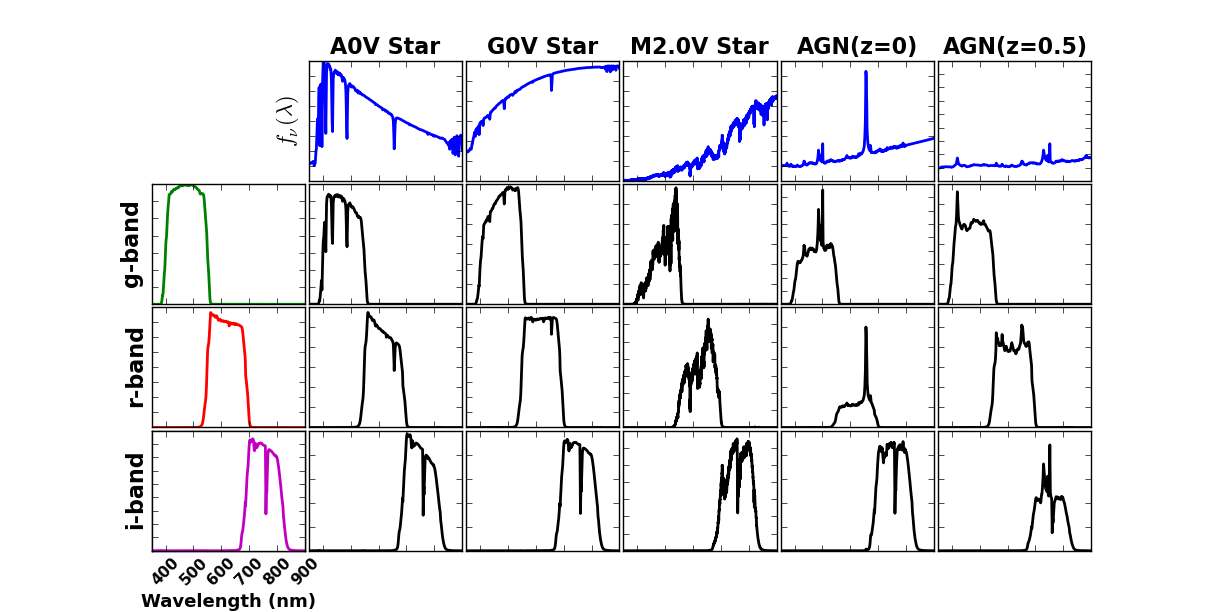
\includegraphics[width=1.1\textwidth]{DCR1.png}
  \caption{{\bf Effective Spectral Energy Distributions} : The
    effective spectra of 5 reference objects -- a ``blue'' {\tt A0V},
    a reference {\tt G0V}, and a ``red'' {\tt M2.0V} star, along with
    a QSO at redshift $z=0$ and $z=0.5$ -- filtered through 3
    transmission profiles corresponding to the LSST $g$, $r$, and
    $i$--bands at 1.2 airmasses.  The top row shows the input spectral
    energy distribution $f_\nu(\lambda)$, while the leftmost column
    shows the LSST filter transmission profile in units of the
    normalized system response $\phi$.  The inner row,column figures
    show the effective spectrum of each SED (along columns) when
    multiplied through the respective filter (along rows).  In all
    subpanels, the x--axis is wavelength.  The {\tt A0V}, {\tt G0V},
    and {\tt M2.0V} spectra correspond to {CAT\_SHARE\_DATA} files
    {\tt kp01\_9750.fits\_g45\_9830.gz}, {\tt
      km20\_6000.fits\_g30\_6020.gz}, and {\tt m2.0Full.dat.gz}
    respectively, and were used as the SEDs of the stars in the W14
    image simulations.  This figure may be recreated using the script
    {\tt python/DCR.py}.}
  \label{fig:spectra}
\end{figure}
\begin{figure}[!t]
  \centering
  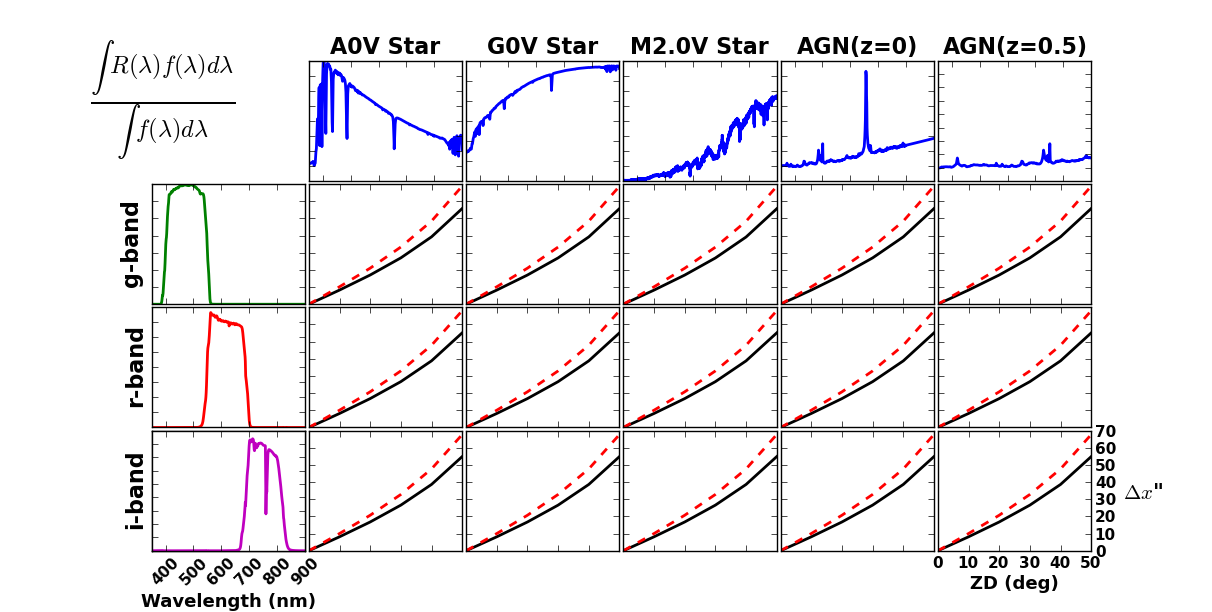
\includegraphics[width=1.1\textwidth]{DCR2.png}
  \caption{{\bf Refraction Amplitude vs. Filter and Spectral Energy
      Distribution}: The flux-weighted amplitude of refraction (in
    arcseconds) for each of the filtered SEDs in
    Figure~\ref{fig:spectra}, as a function of zenith distance in
    degrees along the x--axis.  The solid black line is the nominal
    result from Eqn~\ref{eqn:dcr}, while the dashed red line ignores
    the corrections for temperature and pressure (Eqn~\ref{eqn:dcr0}).
    Note the maximum amplitude of refraction reaches nearly 1
    arcminute.  This figure may be recreated using the script {\tt
      python/DCR.py}.}
  \label{fig:refraction}
\end{figure}

We examined the theoretical amplitude of this effect using discrete
spectra from the {\tt phoSim} source catalog.  We used the same
spectra when generating the images for the pixel--level analysis,
meaning we expect direct agreement between this theoretical analysis
and the expression of DCR in the sims.  In Figure~\ref{fig:spectra},
we show along the top the spectra, in units of $f_\nu(\lambda)$, of 5
sources.  Left to right, these represent a ``blue'' {\tt A0V} star, a
reference {\tt G0V} star, a red {\tt M2.0V} star, and an active
galactic nucleus at redshift $z=0$ and then at $z=0.5$.  We also show
the transmission profiles of the LSST $g$, $r$, and $i$--bands along
the left side of the figure, along with the product of these two
curves which represent the effective spectrum of each source as viewed
through each LSST filter.  Figure~\ref{fig:refraction} shows the
flux--weighted refraction of each SED as a function of zenith
distance.  This is presented in units of arcseconds; note that at the
Universal Cadence limit of $50^{\circ}$ zenith angle, the refraction
of all sources approaches 1 arcminute.  In Figure~\ref{fig:dcr}, we
show the {\it differential} refraction of each spectrum, DCR, with
respect to the {\tt G0V} star.  Note that the maximum amplitude of DCR
is approximately 0.1'' at $50^{\circ}$, or approximately half an LSST
pixel.  This is the effect we wish to explore in this sequence of
analyses.  We included an airmass--dependence to the filter profiles
using the {\tt throughputs} package to yield the flux--weighted DCR
offsets expected for each source in subtask 3, with values listed in
Table~\ref{tab:dcramp}.

\begin{figure}[!t]
  \centering
  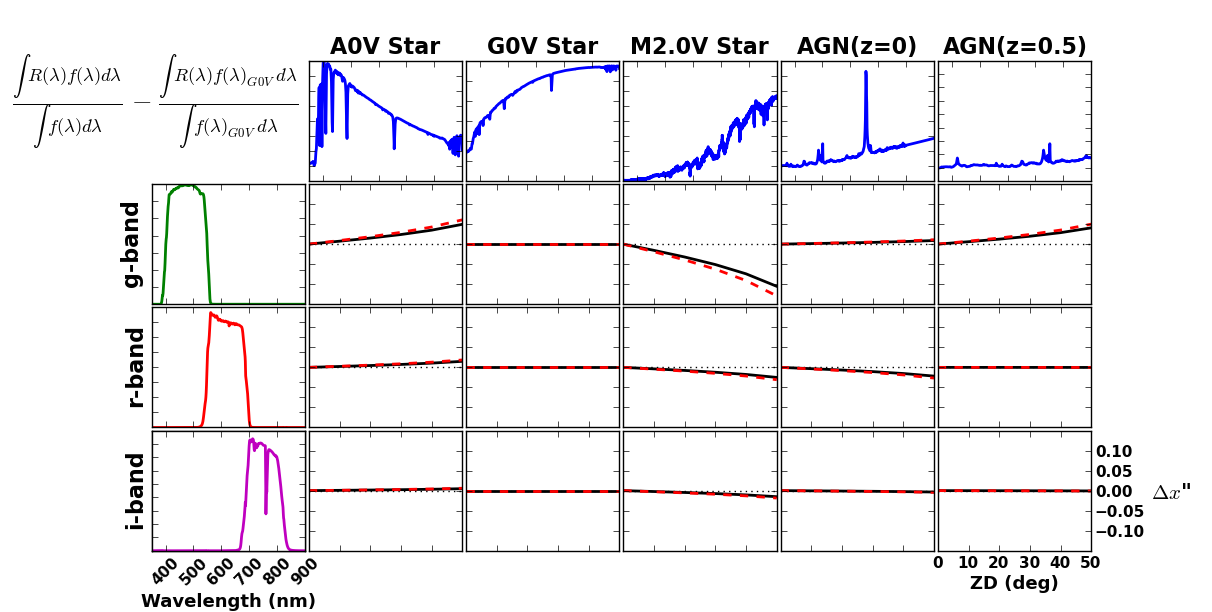
\includegraphics[width=1.1\textwidth]{DCR3.png}
  \caption{{\bf Differential Chromatic Refraction vs. Filter and
      Spectral Energy Distribution}: The differential chromatic
    refraction of all sources from Figure~\ref{fig:spectra} with
    respect to the reference {\tt G0V} star, as a function of zenith
    distance.  The maximum amplitude of DCR between the ``red'' and
    ``blue'' objects reaches $0.2''$, or approximately one LSST pixel.
    This figure may be recreated using the script {\tt
      python/DCR.py}.}
  \label{fig:dcr}
\end{figure}



\section{Results: Subtask 1 \label{sec:task1}}

%To ensure that the results of W14 may be compared to the results from
%W13, we first validated that the {\tt phoSim} software and DM stack
%(and their interaction) had not significantly changed in the interim.
%Unfortunately, we were unable to reproduce the exact simulated images
%from W13 using the version of {\tt phoSim} that was used at the time
%(v3.2.2), even when using the control files that were used as inputs.
%It is unclear exactly why this is the case.  For this reason, we
%up-rev'd to the current v3.3.2 of the {\tt phoSim} software.  Since
%additional features have been added to {\tt phoSim}, and many are
%turned {\bf on} by default, we were again unable to produce an {\it
%  exact} match to the W13 images.  However, we were able to create
%qualitatively similar images by using {\tt phoSim} v3.3.2 and the W13
%control files, with the additional control parameter {\tt
%  fieldanisotropy 0}.  We note that the realized seeing values of the
%images, as measured by the adaptive second moments of the {\tt Psf},
%are systematically ($\sim 5\%$) smaller in the newer data.  This was
%important during the analysis of the deconvolution data, as it
%triggered a bug resolved in Ticket \#3143.

\begin{table}
\centering
\begin{tabular}{ccccc}
\hline
\multicolumn{5}{|c|}{Subtask 1: False Positives in {\tt raft=2,2 sensor=1,1}} \\ \hline \\
Seeing  & Prefilter    & W13  & W14 pipeline on W13 data   & W14   \\
\hline
{\tt 1} & True         & 10   & 10                         & 17    \\
        & False        & 23   & 19                         & 68630 \\
{\tt 2} & True         & 7    & 6                          & 6     \\
        & False        & 8    & 8                          & 6     \\
{\tt 3} & True         & 3    & 3                          & 3     \\
        & False        & 7    & 7                          & 3
\end{tabular}
\caption[]{Summary of the results of subtask 1, which aims to
  reproduce the results of W13 using {\tt phoSim} v3.3.2 and the
  current v7\_3 stack.  The first column shows the numbers of false
  positives from {\tt raft=2,2 sensor=1,1} of the original W13
  analysis, the central column from the re--reduction of those same
  data using the v7\_3 stack, and the final column the results of the
  regenerated images during W14.  The large numbers of false positives
  in the deconvolution configuration (seeing {\tt 1}, prefilter False)
  were triggered by the bug resolved in ticket \#3143.  Results from
  this table were generated using script {\tt
    python/countDiaSourcesT1.py} in this repository.}
\label{tab:task1}
\end{table}

We were unable to reproduce an {\it exact} match to simulated images
from W13, but were able to create qualitatively similar images using
{\tt phoSim} v3.3.2 and the W13 control files, with the additional
control parameter {\tt fieldanisotropy 0}.  We note that the realized
seeing values of the images, as measured by the adaptive second
moments of the {\tt Psf}, are systematically ($\sim 5\%$) smaller in
the newer data.  This was important during the analysis of the
deconvolution data, as it triggered a bug resolved in Ticket \#3143.

We compare the original W13 results, the W13 data run through the W14
pipeline, and the W14 pipeline results in Table~\ref{tab:task1}.  We
first note that the two results running the DM stack on the W13 data
are not exact replicates (first vs. second column). The numbers of
false positives was slightly lower in the newer analysis, especially
in the better seeing data, suggesting minor but noticeable changes in
the algorithms.  The W14 analysis is qualitatively similar, {\it
  except} the configuration that leads to deconvolution of the
template (seeing visit {\tt 1} and no prefiltering).  The moderately
better seeing triggered a bug in the configuration of the
deconvolution kernels, which was resolved in ticket \#3143 and in
subtask 2.  This improvement suggests both that the deconvolution
configuration is currently highly sensitive to the input FWHMs, and
that catastrophic deconvolution failures appear to be potentially
resolvable at the configuration level (i.e. a solution is not
``impossible'').

\section{Results: Subtask 2 \label{sec:task2}}

\begin{table}
\centering
\begin{tabular}{cccc}
\hline
\multicolumn{4}{|c|}{Subtask 2: Average False Positives in {\tt raft=2,2}} \\ \hline \\
Seeing   & Filter & N & N  \\
         &        & Prefilter=False & Prefilter=True   \\
\hline
{\tt 1}  & g      & 2 & 12    \\
{\tt 2}  &        & 7 & 4    \\
{\tt 3}  &        & 4 & 3    \\
\hline
{\tt 1}  & r      & 2 & 8    \\
{\tt 2}  &        & 7 & 5    \\
{\tt 3}  &        & 4 & 3    \\
\hline
{\tt 1}  & i      & 1 & 10    \\
{\tt 2}  &        & 5 & 4    \\
{\tt 3}  &        & 3 & 2    \\
\end{tabular}
\caption[]{Summary of the results of subtask 2.  We show the average
  (over all 9 sensors of raft {\tt 2,2}) of the total number of false
  detections per sensor at 5--sigma, both positive going and negative
  going.  The vast majority of these sources are ``orphans''; the
  average number that associate with a source in the image is less
  than 1 in all cases.  Comparisons of these numbers with theoretical
  expectations are presented in Figure~\ref{fig:fptheory}.  Results
  from this table were generated using script {\tt
    python/countDiaSourcesT2.py} in this repository.}
\label{tab:task2}
\end{table}

%False 4866601 (False,) 9 2 0 2
%True 4866601 (True,) 9 13 0 12
%False 5866601 (False,) 9 2 0 2
%True 5866601 (True,) 9 8 0 8
%False 6866601 (False,) 9 1 0 1
%True 6866601 (True,) 9 10 0 10

%False 4866602 (False,) 9 7 0 7
%True 4866602 (True,) 9 5 0 4
%False 5866602 (False,) 9 7 0 7
%True 5866602 (True,) 9 5 0 5
%False 6866602 (False,) 9 5 0 5
%True 6866602 (True,) 9 4 0 4

%False 4866603 (False,) 9 4 0 4
%True 4866603 (True,) 9 3 0 3
%False 5866603 (False,) 9 4 0 4
%True 5866603 (True,) 9 3 0 3
%False 6866603 (False,) 9 3 0 3
%True 6866603 (True,) 9 2 0 2


\begin{figure}[!h]
  \centering
  \subfloat[Prefiltering = False]{{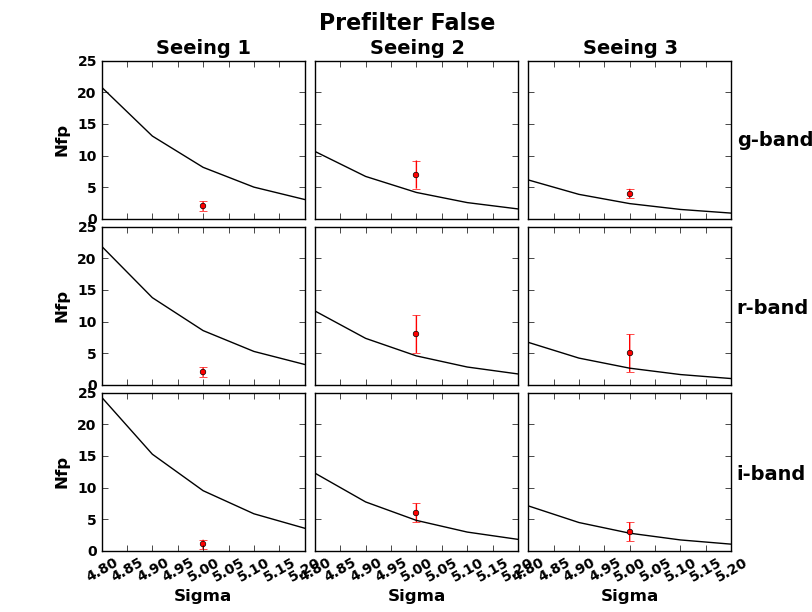
\includegraphics[width=0.65\textwidth]{outputs5b_doPreConvolveFalse_fp.png} }} \\
  \subfloat[Prefiltering = True]{{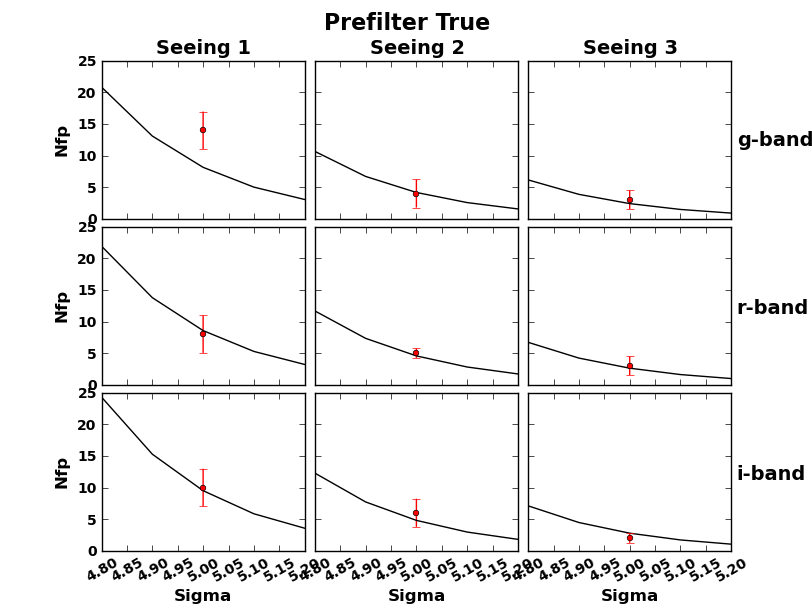
\includegraphics[width=0.65\textwidth]{outputs5b_doPreConvolveTrue_fp.png} }} \\
  \caption{{\bf Subtask 2: False Positive Rates vs. Theory}: Using the
    mean realized seeing for each passband and {\tt Opsim\_rawseeing}
    combination, we plot the expected numbers of false positives per
    sensor (both positive and negative going) as a function of
    detection threshold.  We plot the median number of {\tt
      DiaSources} detected at 5 sigma across the nine {\tt raft=2,2}
    CCDs in red, using the interquartile range to calculate the RMS.
    Results using postfiltering of the data with its {\tt Psf} are on
    the top, and prefiltering are on the bottom.  Note that the
    postfiltering false positives in seeing {\tt 1} which correspond
    to a template deconvolution, are lower than expected due to an
    overestimate of the noise by the variance plane.  The
    postfiltering positives for seeing {\tt 2,3} are consistently
    above the theoretical curve, likely due to a 4--5\% underestimate
    of the noise by the variance plane.  Prefiltering false positives
    appear more evenly distributed above and below the theoretical
    curves.  This figure was created using the script {\tt
      python/falsePositivePlots.py}.}
  \label{fig:fptheory}
\end{figure}

The numbers of false positives in the $gri$--bands are reported in
Table~\ref{tab:task2}.  We averaged over all 9 CCDs in the raft to
report the mean numbers of false positives per CCD.
Figure~\ref{fig:fptheory} compares the number of 5--sigma detected
{\tt DiaSources} in red.  The black line depicts the theoretical run
of false positives with detection threshold, using the mean seeing for
each sample.  We find that, in general, our results are consistent
with this theoretical limit.  One noteworthy exception is in the
deconvolution configuration, where the 0.88'' template is differenced
against the 0.6'' science data without prefiltering (leftmost column
of top panel).  In this case, our realized false positive rate was
significantly {\it lower} than expected from theory.  This is
consistent with the results from W13 (Section 6.4), where
deconvolution significantly enhanced the noise properties of the
difference image.

To quantify this effect in W14, we examined the variance in two ways.
First, we calculated the median value of the difference image variance
plane $V_p$, ignoring any masked pixels.  We then calculated the
empirical variance of the corresponding image plane, scaling its
interquartile range by 0.741 as expected from a Gaussian distribution,
and squared this result to yield $V_e$.  We calculated the ratio
$V_e$/$V_p$ to measure how much the propagated variance
over/underestimates the empirical variance.  We find that the median
of this ratio was within 1\% of 1.0 for all prefiltering and
postfiltering data, {\it including the deconvolution configuration}.
This median value is however consistently above 1.0, indicating slight
underestimation of the true variance by the propagated variance plane
in all cases.  This indicates that the variance plane provides an
adequate estimate of the noise in the image at the stage immediately
following image subtraction.

Secondly, we took the difference images that had {\it not} been
filtered by their {\tt Psf}, and perform the {\tt Psf} convolution.
We note that this is the image that the detection algorithm operates
on in the postfiltering configuration (in fact, this is the
postfiltering process itself!).  In prefiltering, this detection image
is the image difference product itself, which we demonstrated above to
have adequate variance tracking.  We then calculated the same ratios
for this filtered difference image.  We find that for the
deconvolution configurations, the variance plane provided an {\it
  overestimate} of the empirical variance by 30--40\% ($V_e$/$V_p$ =
0.7--0.76).  For the convolution configurations, the variance plane
{\it underestimates} the empirical variance by 4--5\%.  An
overestimate of the variance by 35\% should lead to 15--20 times lower
false positive rate at 5--sigma; a variance underestimate by 5\%
should lead to a false positive rate 2--3 times higher.  These numbers
are roughly consistent with, but larger in amplitude than, empirical
results.  Figure~\ref{fig:fptheory} shows that the {\tt
  prefilter=False} false positives rates are significantly lower than
theory in the prefiltering seeing {\tt 1} data (deconvolution; the
variance plane overestimates the true noise) and moderately but
consistently higher than theory in the seeing {\tt 2,3} data
(convolution; variance plane underestimates the true noise).  As
mentioned in the W13 report, the fact that the template is convolved
twice is thought to be the main reason we have a poor estimate of the
noise at the detection stage in the postfiltering analysis.  For
completeness, we found no filter--dependence to these results.  We
used script {\tt python/examineVariance.py} for this analysis.

\section{Results: Subtask 3 \label{sec:task3}}

\begin{figure}[!ht]
  \centering
  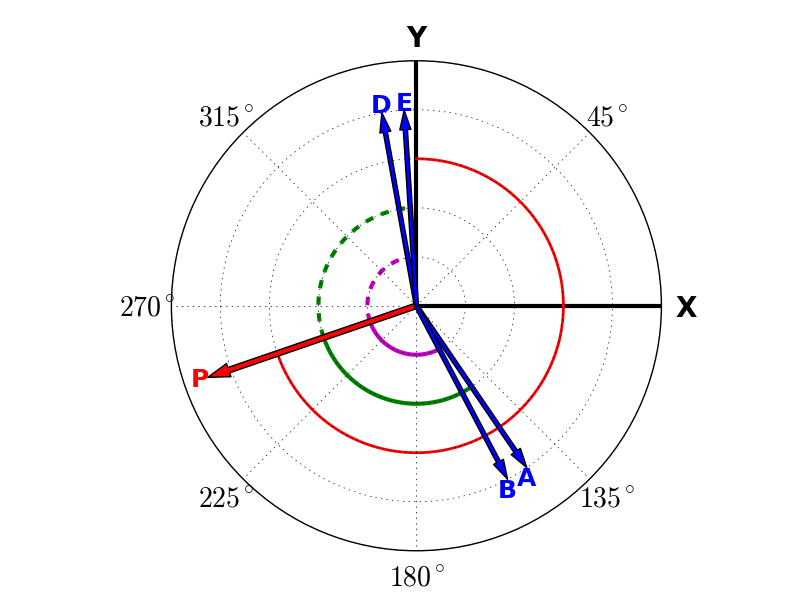
\includegraphics[width=1.1\textwidth]{dcrPhoSim.png}
  \caption{{\bf Designed Orientation of DCR in W14 PhoSim Runs}: This
    figure represents the anticipated orientations of DCR in the W14
    {\tt phoSim} data.  The x,y coordinate system is depicted, as well
    as the convention that angles ({\tt rotTelPos}, {\tt rotSkyPos})
    rotate clockwise with respect to the positive y--axis in the image
    coordinate system (and counterclockwise in the camera coordinate
    system).  The {\tt rotTelPos} of 251 degrees specified for all
    simulations, which reflects the direction to the pole, is shown
    with the red vector \P\ and the red arc at y=0.6.  The derived
    {\tt rotSkyPos} for visits \A,\B,\D,\E\ are shown with the blue
    vectors, and reflect the angle towards zenith (the angle of
    increasing altitude).  DCR is expected to happen along these
    vectors.  The angles \P\A,\P\E\ are similar, and represented by
    the green arcs at y=0.4; the angles \P\B,\P\D\ are also similar,
    and represented by the purple arcs at y=0.2.  This is expected as
    observations \A\ and \E\ are taken at airmass 1.55 (zenith
    distance of 50 degrees) but at opposite sides of the meridian
    crossing of the star field; a similar situation was designed for
    observations \B\ and \D, which are taken at airmass 1.16 (zenith
    distance of 30 degrees).  Visit \C\ is not depicted as it was
    taken at zenith.  This figure was created using the script {\tt
      python/dcrSchematic.py}.}
  \label{fig:phosimdcr}
\end{figure}

Figure~\ref{fig:phosimdcr} demonstrates the designed directions of
increasing altitude (orientation of blue--source positive dipoles due
to DCR) in visits \A, \B, \D, and \E\ (visit \C\ is effectively at
zenith and thus no DCR is expected).  These are set by {\tt phoSim}
configuration parameter {\tt rotTelPos}.  The direction to the pole is
also indicated, and set by {\tt phoSim} configuration parameter {\tt
  rotSkyPos}.  For reference, {\tt rottelpos} is defined as ({\tt
  rotskypos}-180+parallactic angle), such that the angle of DCR should
be along this axis.  The numerical values of these angles, measured
clockwise with respect to the positive y--axis (i.e. ``up'') are
listed in the first numerical column of Table~\ref{tab:dcrang}.  The
per--spectrum and per--passbands expected amplitudes of the DCR shift,
w.r.t. the {\tt G0V} stars, are given in the first numerical column of
Table~\ref{tab:dcramp}.

\subsection{Dipole Orientation and Amplitude}

\begin{figure}
    \centering
    \subfloat[Visit A]{{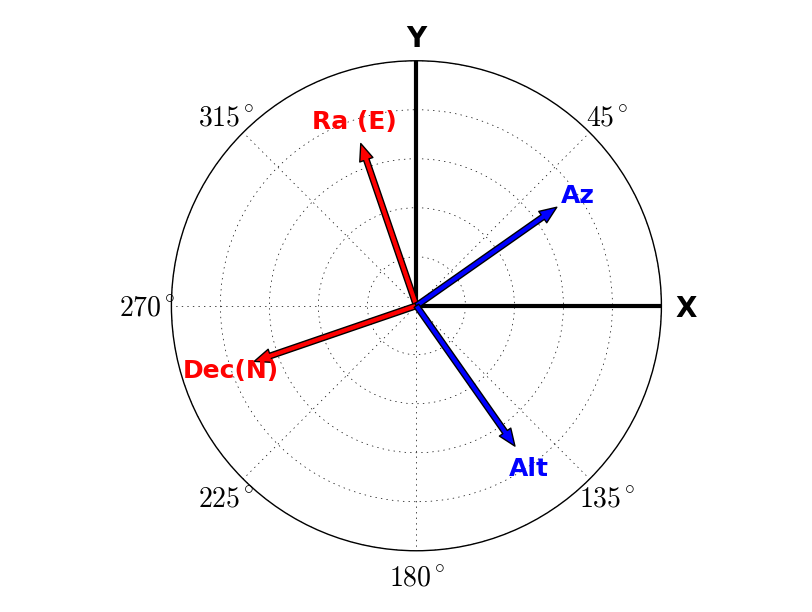
\includegraphics[width=0.46\textwidth]{outputs8bCA_dcr_wcs.png} }}
    \qquad
    \subfloat[Visit B]{{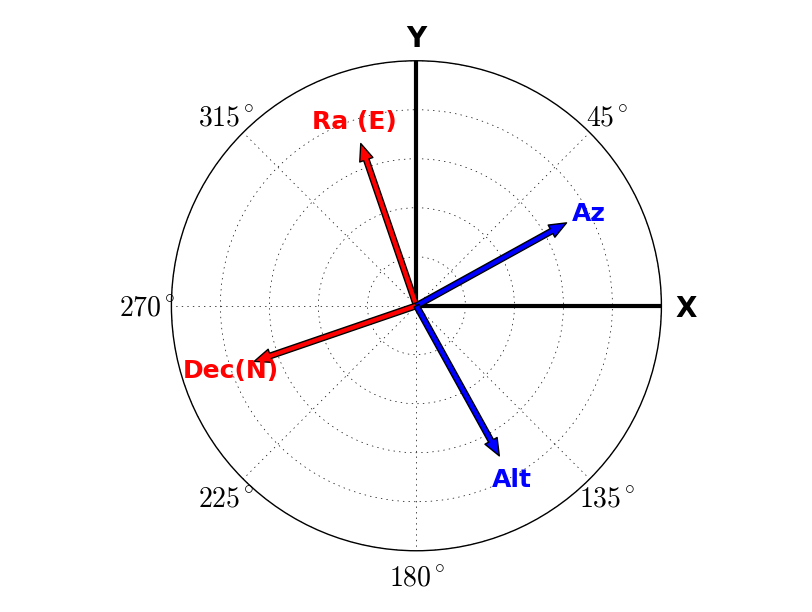
\includegraphics[width=0.46\textwidth]{outputs8bCB_dcr_wcs.png} }} \\
    \subfloat[Visit D]{{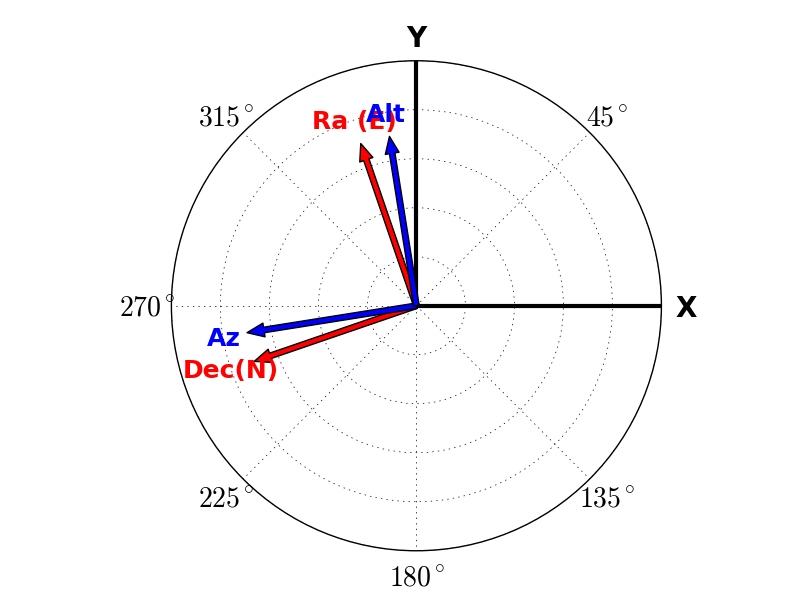
\includegraphics[width=0.46\textwidth]{outputs8bCD_dcr_wcs.png} }}
    \qquad
    \subfloat[Visit E]{{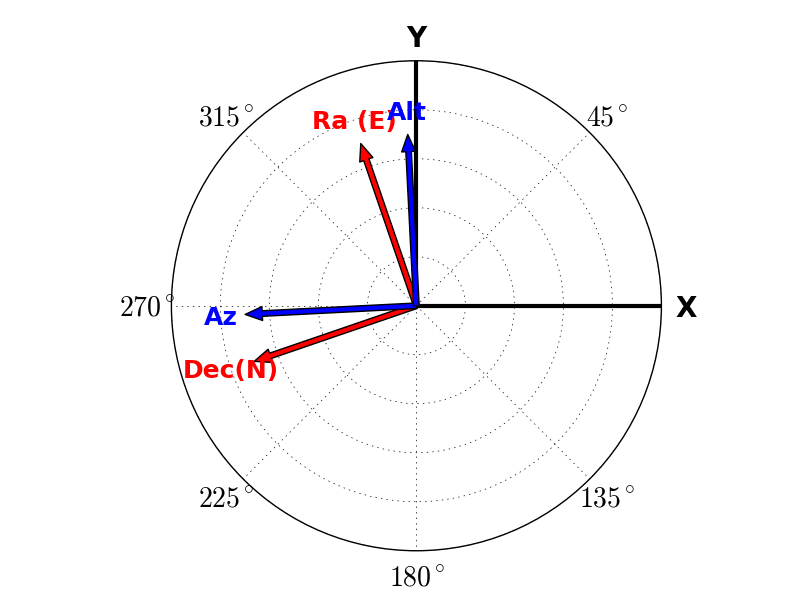
\includegraphics[width=0.46\textwidth]{outputs8bCE_dcr_wcs.png} }} \\
    \caption{{\bf Wcs-Derived Orientations of PhoSim Data}: These
      figures show the orientations of the Right Ascension and
      Declination axes (red), and Azimuth and Altitude axes (blue) of
      visits \A,\B,\D,\E.  Arrows represent the directions of {\it
        increasing} coordinate value.  The Ra,Dec axes are the same in
      all images since they were designed to have a common {\tt
        rotTelPos}.  Ideally, the directions of increasing Alt will
      correspond to the {\tt rotSkyPos} depicted in
      Figure~\ref{fig:phosimdcr}.  All coordinate system orientations
      were derived from the fitted Wcs of the {\tt calexp} of the
      $g$--band observation of seeing {\tt 2} data.  To determine the
      orientations empirically, small steps were taken in each
      coordinate starting at the center of the image, and the {\tt
        Wcs} and topocentric corrections used to map these back into
      offsets in the pixel plane.  This figure was created using the
      script {\tt python/compareDcrFromSims.py}.}
    \label{fig:wcsdcr}
\end{figure}

Our first validation of DCR comes from looking at the fitted {\tt Wcs}
of each {\tt calexp} to establish directionality.  Using a topocentric
correction and the requested times of observation, we empirically
determined the angles of increasing Ra,Dec and Az,Alt by taking 10''
steps along each axis, starting at the field center, and converting
these coordinate steps to pixel offsets.  These axes are represented
in Figure~\ref{fig:wcsdcr} for visits \A\B\D\E, and the numerical
values of the angle of increasing Altitude are provided in the second
column of Table~\ref{tab:dcrang}.  We note that these angles are
similar to the requested {\tt rotTelPos}, typically to within a
degree.

\begin{table}
\centering
\begin{tabular}{ccccc}
\hline
\multicolumn{5}{|c|}{Subtask 3: Orientation of DCR} \\ \hline \\
Visit    & SED & {\tt rotTelPos} & {\tt Wcs} + Topo & Measured \\
         &     &                 &                  & Dipole Orientation \\
\hline
\A & {\tt A0V}   & $145.7^{\circ}$ & $144.9^{\circ}$ & $145.7^{\circ}$    \\
   & {\tt M2.0V} & $325.7^{\circ}$ & $324.9^{\circ}$ & $325.6^{\circ}$    \\
\hline
\B & {\tt A0V}   & $152.3^{\circ}$ & $151.1^{\circ}$ & $151.7^{\circ}$    \\
   & {\tt M2.0V} & $332.3^{\circ}$ & $331.1^{\circ}$ & $331.8^{\circ}$    \\
\hline
\D & {\tt A0V}   & $349.9^{\circ}$ & $351.0^{\circ}$ & $349.3^{\circ}$    \\
   & {\tt M2.0V} & $169.9^{\circ}$ & $171.0^{\circ}$ & $170.0^{\circ}$    \\
\hline
\E & {\tt A0V}   & $356.4^{\circ}$ & $357.1^{\circ}$ & $355.2^{\circ}$    \\
   & {\tt M2.0V} & $176.4^{\circ}$ & $177.1^{\circ}$ & $176.2^{\circ}$    \\
\end{tabular}
\caption[So I can have 2 paragraphs]{The expected and measured
  orientations of DCR, using the coordinate conventions depicted in
  Figure~\ref{fig:phosimdcr}.  These numbers represent the orientation
  of the {\it positive} lobe of any dipole arising from the DCR effect
  for blue sources, and reflect the angle of increasing altitude.
  Numbers are reported as a function of visit \A\B\D\E, and the
  spectral energy distribution of the source.  The numbers under {\tt
    rotTelPos} reflect the designed orientation of DCR that was input
  to {\tt phoSim}.  The numbers under {\tt Wcs} reflect the
  empirically determined direction to zenith in each image, using the
  {\tt calexp} fitted {\tt Wcs} and topocentric corrections
  appropriate for each visit.  Finally, we report the measured median
  orientation of DiaSources in each image difference, when differenced
  against the template taken at zenith (visit \C).  For the {\tt
    rotTelPos} and {\tt Wcs} columns, the numbers for the red {\tt
    M2.0V} stars are simply $180^{\circ}$ from those of the blue {\tt
    A0V} stars.  For the orientation column, we use fitted values from
  $g$--band data, seeing {\tt 1} (dipole results in the $r$--band show
  quantitatively similar results).  We also find no dependence of
  these orientations on seeing.  We only report these numbers using
  the postfiltered data, where dipole measurement is known to operate
  correctly.  Full results may be found in the file {\tt NOTES}.}
\label{tab:dcrang}
\end{table}

\begin{table}
\centering
\begin{tabular}{cccccccc}
\hline
\multicolumn{8}{|c|}{Subtask 3: Amplitude of DCR} \\ \hline \\
Visit    & SED & Filter & Theory & {\tt Wcs} Offsets & Dipole Fit         & Dipole Fit         & Dipole Fit \\
         &     &        &        &                   & Seeing Bin {\tt 1} & Seeing Bin {\tt 2} & Seeing Bin {\tt 3} \\
\hline
\A & {\tt A0V}   & $g$ & 0.0406'' & 0.0421$\pm$0.0014'' & 0.167''  & 0.259''  & 0.208''  \\
   &             & $r$ & 0.0125'' & 0.0129$\pm$0.0005'' & 0.049''  & $\cdots$ & $\cdots$ \\
   &             & $i$ & 0.0040'' & 0.0044$\pm$0.0005'' & $\cdots$ & $\cdots$ & $\cdots$ \\
   & {\tt M2.0V} & $g$ & 0.0862'' & 0.0768$\pm$0.0029'' & 0.144''  & 0.204''  & 0.293''  \\
   &             & $r$ & 0.0207'' & 0.0199$\pm$0.0007'' & 0.230''  & $\cdots$ & $\cdots$ \\
   &             & $i$ & 0.0125'' & 0.0120$\pm$0.0008'' & $\cdots$ & $\cdots$ & $\cdots$ \\
\hline
\B & {\tt A0V}   & $g$ & 0.0199'' & 0.0205$\pm$0.0008'' & 0.183''  & 0.243''  & $\cdots$ \\
   &             & $r$ & 0.0060'' & 0.0064$\pm$0.0007'' & $\cdots$ & $\cdots$ & $\cdots$ \\
   &             & $i$ & 0.0019'' & 0.0023$\pm$0.0004'' & $\cdots$ & $\cdots$ & $\cdots$ \\
   & {\tt M2.0V} & $g$ & 0.0424'' & 0.0385$\pm$0.0012'' & 0.222''  & 0.266''  & $\cdots$ \\
   &             & $r$ & 0.0101'' & 0.0099$\pm$0.0007'' & $\cdots$ & $\cdots$ & $\cdots$ \\
   &             & $i$ & 0.0061'' & 0.0056$\pm$0.0008'' & $\cdots$ & $\cdots$ & $\cdots$ \\
\hline
\D & {\tt A0V}   & $g$ & 0.0199'' & 0.0200$\pm$0.0008'' & 0.201''  & 0.251''  & $\cdots$ \\
   &             & $r$ & 0.0060'' & 0.0062$\pm$0.0006'' & $\cdots$ & $\cdots$ & $\cdots$ \\
   &             & $i$ & 0.0019'' & 0.0025$\pm$0.0005'' & $\cdots$ & $\cdots$ & $\cdots$ \\
   & {\tt M2.0V} & $g$ & 0.0424'' & 0.0385$\pm$0.0010'' & 0.201''  & 0.254''  & $\cdots$ \\
   &             & $r$ & 0.0101'' & 0.0097$\pm$0.0006'' & $\cdots$ & $\cdots$ & $\cdots$ \\
   &             & $i$ & 0.0061'' & 0.0057$\pm$0.0008'' & $\cdots$ & $\cdots$ & $\cdots$ \\
\hline
\E & {\tt A0V}   & $g$ & 0.0406'' & 0.0430$\pm$0.0027'' & 0.169''  & 0.235''  & 0.360''  \\
   &             & $r$ & 0.0125'' & 0.0127$\pm$0.0004'' & 0.135''  & $\cdots$ & $\cdots$ \\
   &             & $i$ & 0.0040'' & 0.0049$\pm$0.0007'' & $\cdots$ & $\cdots$ & $\cdots$ \\
   & {\tt M2.0V} & $g$ & 0.0862'' & 0.0771$\pm$0.0022'' & 0.158''  & 0.213''  & 0.267''  \\
   &             & $r$ & 0.0207'' & 0.0197$\pm$0.0006'' & 0.262''  & $\cdots$ & $\cdots$ \\
   &             & $i$ & 0.0125'' & 0.0115$\pm$0.0010'' & $\cdots$ & $\cdots$ & $\cdots$ \\
\end{tabular}
\caption[So I can have 2 paragraphs]{The expected and measured
  amplitudes of DCR, in arcseconds.  These numbers represent the
  differential offset between positions of an object at zenith (visit
  \C) and at the airmasses associated with visits \A\B\D\E, with
  respect to the positions of the reference {\tt G0V} stars, which
  define the astrometric reference system in this study.  The Theory
  column is the expected amplitude as described in
  Section~\ref{sec:theory}, using airmass--dependent filter profiles,
  atmospheric water vapor pressure of $f=8$ mmHg, ambient air pressure
  of $P$ = 520 mmHg, and ground temperature of $T=20$ C.  The {\tt
    Wcs} column represents the median (over all seeing values and
  sensors) offsets between stars of the given SED and the astrometric
  reference solution, determined using the {\tt Wcs} and {\tt Source}
  products.  Results in all passbands are consistent with zero
  refraction for the \C\C\ visits (within 0.001'').  We find moderate
  airmass dependence of the {\tt G0V} star residuals with an amplitude
  of 0.002'', 0.0005'', and 0.0006'' in the $g,r,i$--bands,
  respectively.  The mean dipole amplitudes are determined using the
  same fits that yield the dipole orientations in
  Table~\ref{tab:dcrang}, and represent the offset between the fitted
  positive and negative lobes of the dipole.  Because we see a seeing
  dependence on these numbers, we report them for each of the seeing
  bins {\tt 1,2,3}.  Theory results were determined using script {\tt
    python/DCR2.py}.  Astrometric residuals were determined using
  script {\tt astrometricResids.py}.  Full results may be found in the
  file {\tt NOTES}.}
\label{tab:dcramp}
\end{table}

Our second validation of DCR comes from looking at the astrometric
residuals of the stars with respect to the reference catalog, after
fitting for the {\tt Wcs} model.  We grouped the stars into 3 bins
based upon their SED.  We then calculated the mean amplitude of
residuals to the astrometric fit, which is driven by the {\tt G0V}
stars.  The second numerical column of Table~\ref{tab:dcramp} provides
this information.  We note that the DCR amplitudes for the {\tt A0V}
objects are roughly consistent with theory, although uniformly
over--refracted by $\sim 4\%$.  The amplitudes of the relative
refraction of the {\tt M2.0V} objects are under--refracted but by
$\sim 10\%$.  The expected trend of the ``red'' star DCR amplitude
being larger than the ``blue'' stars amplitude, as depicted in
Figure~\ref{fig:dcr}, is seen here.

Finally, we compared the measurements of dipoles in the difference
images to the expected effects of DCR.  For this analysis, we only
looked at difference images where the template image comes from zenith
(i.e. visit \C).  The joint--Psf dipole measurement model
simultaneously fits for a positive--going and negative--going
component of the source -- a 6--parameter fit including 2 centroids
and 2 fluxes.  The separation of the positive--going and
negative--going component are proxies for the DCR effect.  We used
measurements from the postfiltered data only because the measurement
suite is not fully implemented for prefiltered data.  Because we found
the most dipoles in the $g$--band seeing {\tt 1} data, we used these
measurements to validate the DCR orientation.  The orientation numbers
are presented in the third numerical column of Table~\ref{tab:dcrang}.
We find that these numbers are also consistent with the designed
orientation to within approximately $1^{\circ}$.  We find no seeing
dependence on these values.

The passband--dependent separations of the dipole lobes are given in
the final columns of Table~\ref{tab:dcramp}, again only using the data
differenced against template visit \C.  We find that these values are
considerably larger than the DCR amplitude expected from theory, and
from the amplitudes suggested by the {\tt Wcs} residuals.
Additionally, we find that this overestimate is a function of seeing,
in the sense that in the worse seeing data these values are typically
overmeasured by a larger degree.  This a strong indication that there
are aspects of the dipole measurement algorithm that need to be
improved upon.  We only found significant numbers of dipoles in the
$r$--band data in the data at airmass 1.55.  For the $i$--band data,
there were not enough dipoles in any conditions to provide a
measurement.

\subsection{Dipole Rate}


\begin{figure}[!ht]
  \centering
  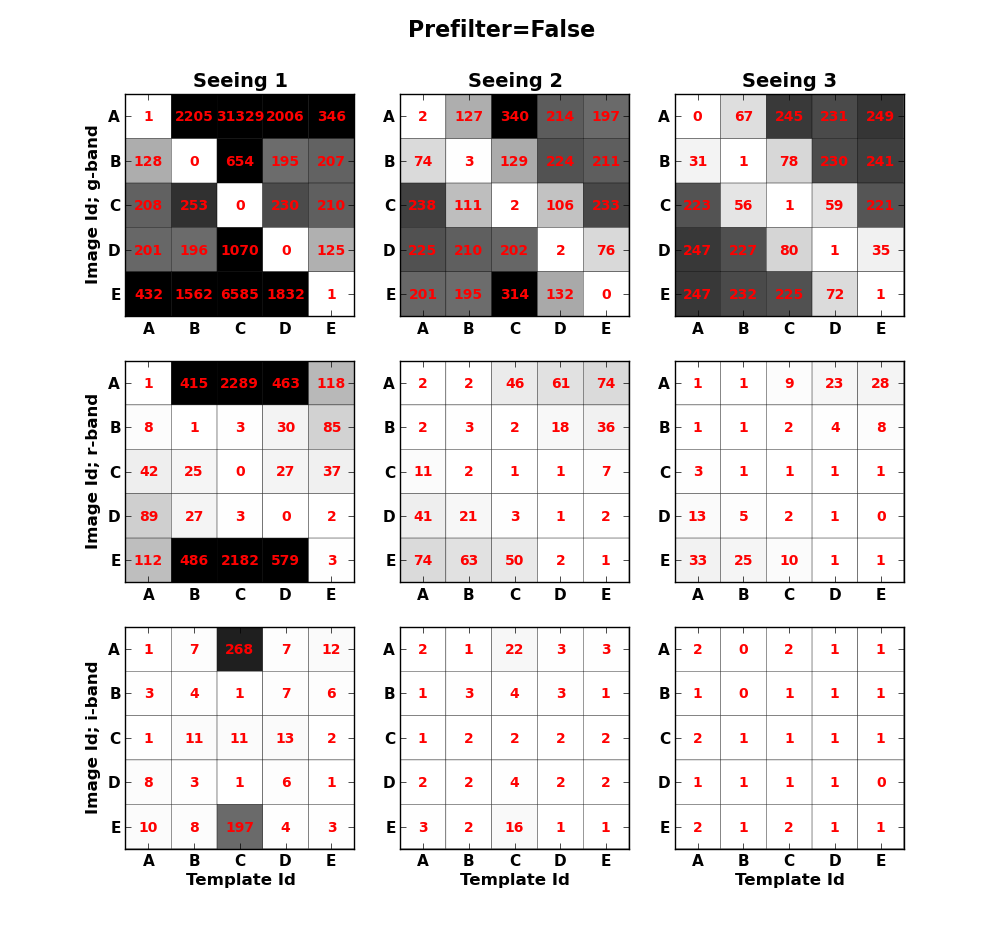
\includegraphics[width=1.0\textwidth]{heatmapFalse.png}
  \caption{{\bf Number of False Positives, Postfiltering}: This figure
    shows the median number of false positives across the nine {\tt
      raft=2,2} CCDs.  The first row of information shows these
    ``heat-maps'' for $g$--band data, the second for $r$--band, and
    the third for $i$--band.  The first column represents the
    good--seeing images, the second the medium--seeing images (same
    quality as template), and the third the poor-seeing images.
    Within each filter--seeing combination, the heat--map represents
    the median number of false positives as a function of the image
    airmass (visit \A\B\C\D\E) along the y--axis, and template airmass
    (visit \A\B\C\D\E) along the x--axis.  The diagonal elements
    represent the situation where the template and science image are
    taken at the same airmass and have the same orientation
    w.r.t. zenith.  The off--diagonal elements represent a mismatch
    between the template and science image in terms of airmass and/or
    parallactic angle.  The general trend is that the numbers of false
    positives decrease with decreasing differences in the
    airmass,angle attributes of the template and science image,
    decrease with increasing seeing, and decrease with increasing
    wavelength.  The $i$-band data in poor seeing do not appear
    sensitive to DCR.  This figure was created using the script {\tt
      python/heatMap.py}.}
  \label{fig:heatpost}
\end{figure}

\begin{figure}[!ht]
  \centering
  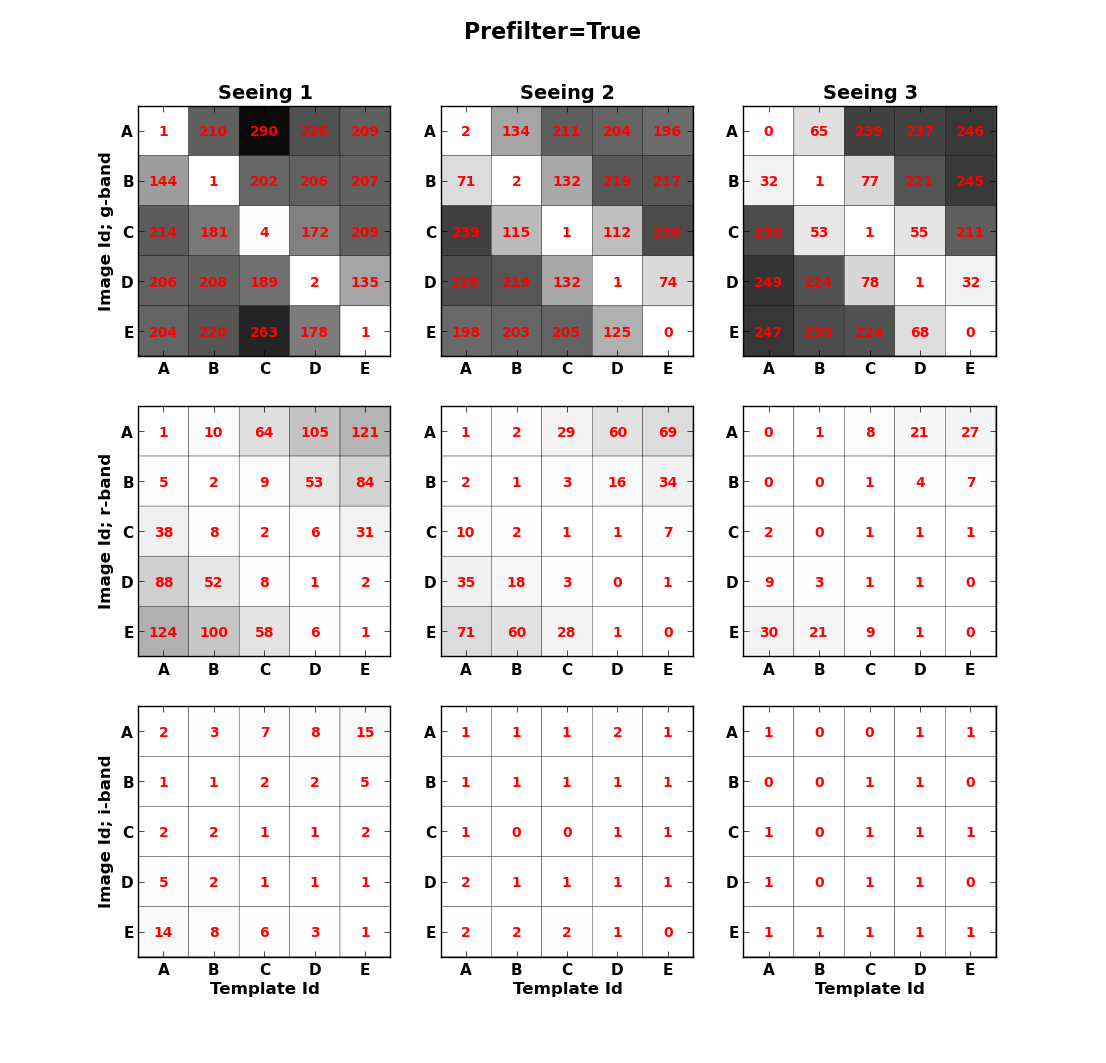
\includegraphics[width=1.0\textwidth]{heatmapTrue.png}
  \caption{{\bf Number of False Positives, Prefiltering}: Same as
    Figure~\ref{fig:heatpost}, but using prefiltering of the science
    image with its Psf.  The numbers of false positives is generally
    lower than in the postfiltering case (Figure~\ref{fig:heatpost}).
    This figure was created using the script {\tt python/heatMap.py}.}
  \label{fig:heatpre}
\end{figure}

Figures~\ref{fig:heatpost} and \ref{fig:heatpre} show the median
number of false positives per CCD within raft {\tt 2,2}.  These are
given as a function of passband, and science visit vs. template visit.
The ``on--axis'' elements within each matrix represent configurations
where DCR within the template and science image are exactly aligned.
These values are consistent with the results seen in subtasks 1 and 2,
indicating that DCR is an effect that may be compensated for when
realized similarly in a template and science image.

The off axis elements correspond to a mismatch between template and
science image conditions, and show an enhanced rate of false
positives.  This enhancement is strongest in the $g$--band, and in the
better seeing data.  The number of false positives is also
significantly smaller in the prefiltering data.  Importantly, when the
airmasses are similar but the parallactic angle through the images
different, an enhanced rate of false positives is seen, suggesting
that the image subtraction template suite must accommodate orientation
as well as airmass.  We elaborate on this in
Section~\ref{sec:templates}.  The effects of mismatched parallactic
angles are mostly negligible in the $i$--band data, except in the best
seeing conditions.  However, for the majority of the $g$ and $r$--band
(and presumably $u$--band) data, DCR appears to be a significant
impediment to achieving a noise--limited false positive rate.

There are 2 apparent components to the heat maps.  The first
corresponds to an enhancement in the rate of the no--refraction to
high--refraction differences (\C\A\ and \C\E), which show large
numbers of false positives in good seeing, and in the prefiltering
data appears localized to the $g$--band data.  The second component
corresponds to the maximal mismatch between the DCR vector (\A\E\ and
\E\A), and appears to be the dominant mode in the worse seeing data,
in the redder passbands, and in the non--$g$--band prefiltering data.

\section{Implications for Image Subtraction Templates \label{sec:templates}}

We examine the implications for the image subtraction template suite,
using the observed correlation between DCR amplitude and false positive
rate.

We first look at the number of false positives when differencing
against the zenith template \C.  We associated these false positives
with the reference catalog, and binned them based upon the SED they
match to.  We then normalize each of these populations by the number
that are expected from background fluctuations.  We plot these values
against the measured DCR offsets (using the WCS--based analysis from
Table~\ref{tab:dcramp}), in units of the PSF FWHM, in
Figure~\ref{fig:fpregress}.  Data from the {\tt A0V} stars are plotted
in blue, and from the {\tt M2.0V} stars in red.  We use information
from all passbands and all seeings on this plot; the seeing {\tt
  1,2,3} data are encoded as circles, squares, and triangles,
respectively.

We fit a linear regression to each curve of the form $log_{10}~y = a +
b * log_{10}~x$, finding:
\begin{eqnarray}
%A-star True:  logy = 4.5207 + 2.2470 logx.  logy=0 at x=0.0097
%A-star False: logy = 5.5313 + 2.7537 logx.  logy=0 at x=0.0098
{\tt A0V}   & {\rm Prefilter=True}  & log_{10}~y = 4.52 + 2.25 ~log_{10}~x \\ \nonumber
            & {\rm Prefilter=False} & log_{10}~y = 5.53 + 2.75 ~log_{10}~x \\ \nonumber
%M-star True:  logy = 4.5773 + 2.6279 logx.  logy=0 at x=0.0181
%M-star False: logy = 4.7113 + 2.6713 logx.  logy=0 at x=0.0172
{\tt M2.0V} & {\rm Prefilter=True}  & log_{10}~y = 4.58 + 2.63 ~log_{10}~x \\ \nonumber
            & {\rm Prefilter=False} & log_{10}~y = 4.71 + 2.67 ~log_{10}~x
\end{eqnarray}
We plot these as the solid lines in Figure~\ref{fig:fpregress}.  The
curves are significantly different for the red and blue stars, which
is not entirely understood at this time.  We naively expect the curves
to look the same since we are effectively including information about
the spectral type in the amplitude of the DCR shift, along the {\tt
  x}--axis.  It is possible that these difference come from
second--order color effects in the sims, including color--dependent
shape and size of the PSF.  Vertical lines are plotted where these
curves cross {\tt y=1}, which effectively represents a doubling of the
false positive rate due to DCR from each class of stars.  We find that
the prefiltering and postfiltering lines cross at essentially the same
value, amplitude/FWHM = 0.01 and 0.02 for the {\tt A0V} and {\tt
  M2.0V} stars, respectively.  For a fiducial seeing value of $0.6''$,
this means that DCR begins to dominate the false positive rate at DCR
amplitudes of 6--11 mas.  At $0.88''$, similar rates will be seen at
DCR amplitudes of 9--16 mas.

We repeat the above analysis normalizing by the number of stars in
each image, which typically number 80--90 for the {\tt A0V} and {\tt
  M2.0V} stars.  This provides the likelihood that a given object will
lead to a false positive as a function of DCR offset, for objects in
our S/N range (100--200).  We regress using the same functional form
as above and find:
\begin{eqnarray}
%A-star True:  logy = 2.7165 + 2.0063 logx.  logy=-2 at x=0.0045
%A-star False: logy = 4.0737 + 2.7322 logx.  logy=-2 at x=0.0060
{\tt A0V}   & {\rm Prefilter=True}  & log_{10}~y = 2.72 + 2.01 ~log_{10}~x \\ \nonumber
            & {\rm Prefilter=False} & log_{10}~y = 4.07 + 2.73 ~log_{10}~x \\ \nonumber
%M-star True:  logy = 3.0538 + 2.5494 logx.  logy=-2 at x=0.0104
%M-star False: logy = 3.1761 + 2.5848 logx.  logy=-2 at x=0.0099
{\tt M2.0V} & {\rm Prefilter=True}  & log_{10}~y = 3.05 + 2.55 ~log_{10}~x \\ \nonumber
            & {\rm Prefilter=False} & log_{10}~y = 3.18 + 2.58 ~log_{10}~x
\end{eqnarray}
where now $log~y$ represents the log--likelihood that a given object
will yield a false positive.  These curves cross the 1\% likelihood
mark at $x \sim 0.005, 0.01$ for the {\tt A0V} and {\tt M2.0V} stars,
respectively, corresponding to DCR shifts of 3 and 6 mas at $0.6''$
seeing, and 5 and 9 mas in $0.88''$ seeing.  These results are shown in
Figure~\ref{fig:fpregress2}.

We next examined the consequences of this on the airmass and
parallactic angle requirements for image subtraction templates.  We
first calculated the DCR for each source star at fiducial template
airmasses of 1.0 and 1.25, corresponding to the first leg of a
triangle.  A second leg is calculated by considering the amplitude
{\it and} orientation of DCR at a range of other airmasses from
1..1.5, and orientation differences from 1..180 degrees.  This second
airmass is used to calculate the length of the second leg of the
triangle, corresponding to a second realization of DCR in a science
image.  The opening angle between theses two vectors is set to 0..180
degrees in steps of 5, and represents the mismatch between the
parallactic angle in the template and science images.  We use the law
of cosines to describe the astrometric offset $\Delta r$ between the two
apparitions of the source (at the reference airmass, and at all other
combinations of airmass and parallactic angle).  The geometric basis
for this analysis is presented in Figure~\ref{fig:fpgeom}.

The overall offset $\Delta r$ is used to color--code the panels in
Figure~\ref{fig:fpsummary}, which show relative DCR amplitude as a
function of airmass along the {\tt y}--axis, and difference in the
parallactic angle along the {\tt x}--axis.  We overplot lines of
constant offset at 3 (blue solid line) and 6 (red dashed line) mas,
corresponding to the approximate DCR offsets that yield 1\% likelihood
of dipoles in 0.6'' seeing for the {\tt A0V} and {\tt M2.0V} stars,
respectively.  The top panel shows these results for a template at
airmass 1.0, which has no DCR in any passband.  Thus observations at
{\it all} orientations yield similar results, and there is only a rate
dependence on airmass difference.  On the top left we show these
results for the $g$--band, where the amplitudes are all larger than
6mas and thus no contours displayed.  At top middle we show the same
plots for $r$--band templates, which show 6mas relative DCR against
airmass 1.05 to 1.15 science images, and on the top right for
$i$--band which show 6mas relative DCR at airmass 1.15 for the red
stars and 3mas relative DCR at airmass 1.35 for the blue stars.

The bottom panels show these same results for airmass 1.25 templates,
and demonstrate the interaction between airmass and orientation
difference.  For data taken at the same airmass, orientation
differences of 15--25 degrees will yield to 3mas relative DCR in
$r$--band (lower middle), and 20--65 degrees in $i$--band (lower
right), driven by the red stars.  At the same DCR orientation, airmass
differences of approximately 0.1 in $r$--band and 0.15--0.2 in
$i$--band will yield the same enhanced rate of false positives.  We
note that at the coarseness of this study (steps of 0.1 in airmass and
5 degrees in orientation), nearly {\it all} $g$--band data will show
enhanced dipole rates.  This will be seen to a larger degree in the
$u$--band, although the faintness of the redder stars may mean that
there will be fewer red objects in the images, and accordingly a bluer
astrometric reference frame used.

\begin{figure}[!ht]
  \centering
  \subfloat[Prefiltering = False]{{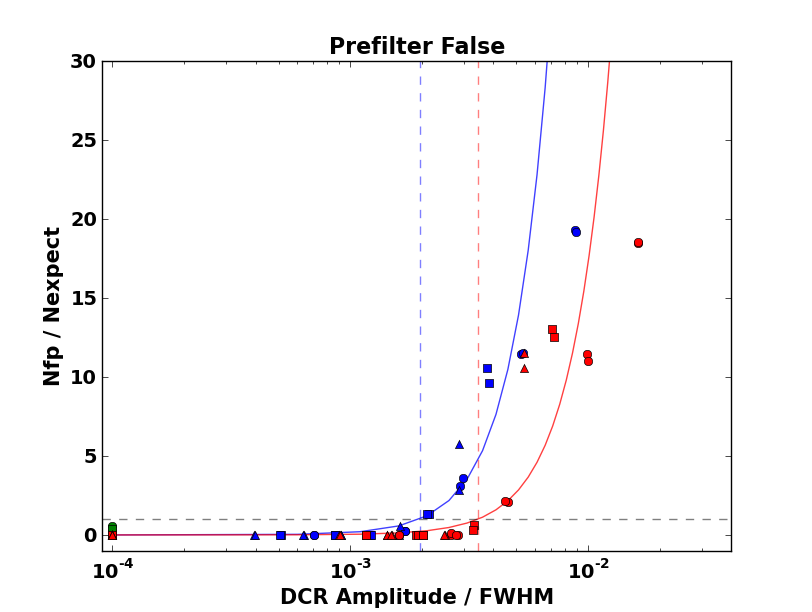
\includegraphics[width=0.65\textwidth]{regressFalse.png} }} \\
  \subfloat[Prefiltering = True]{{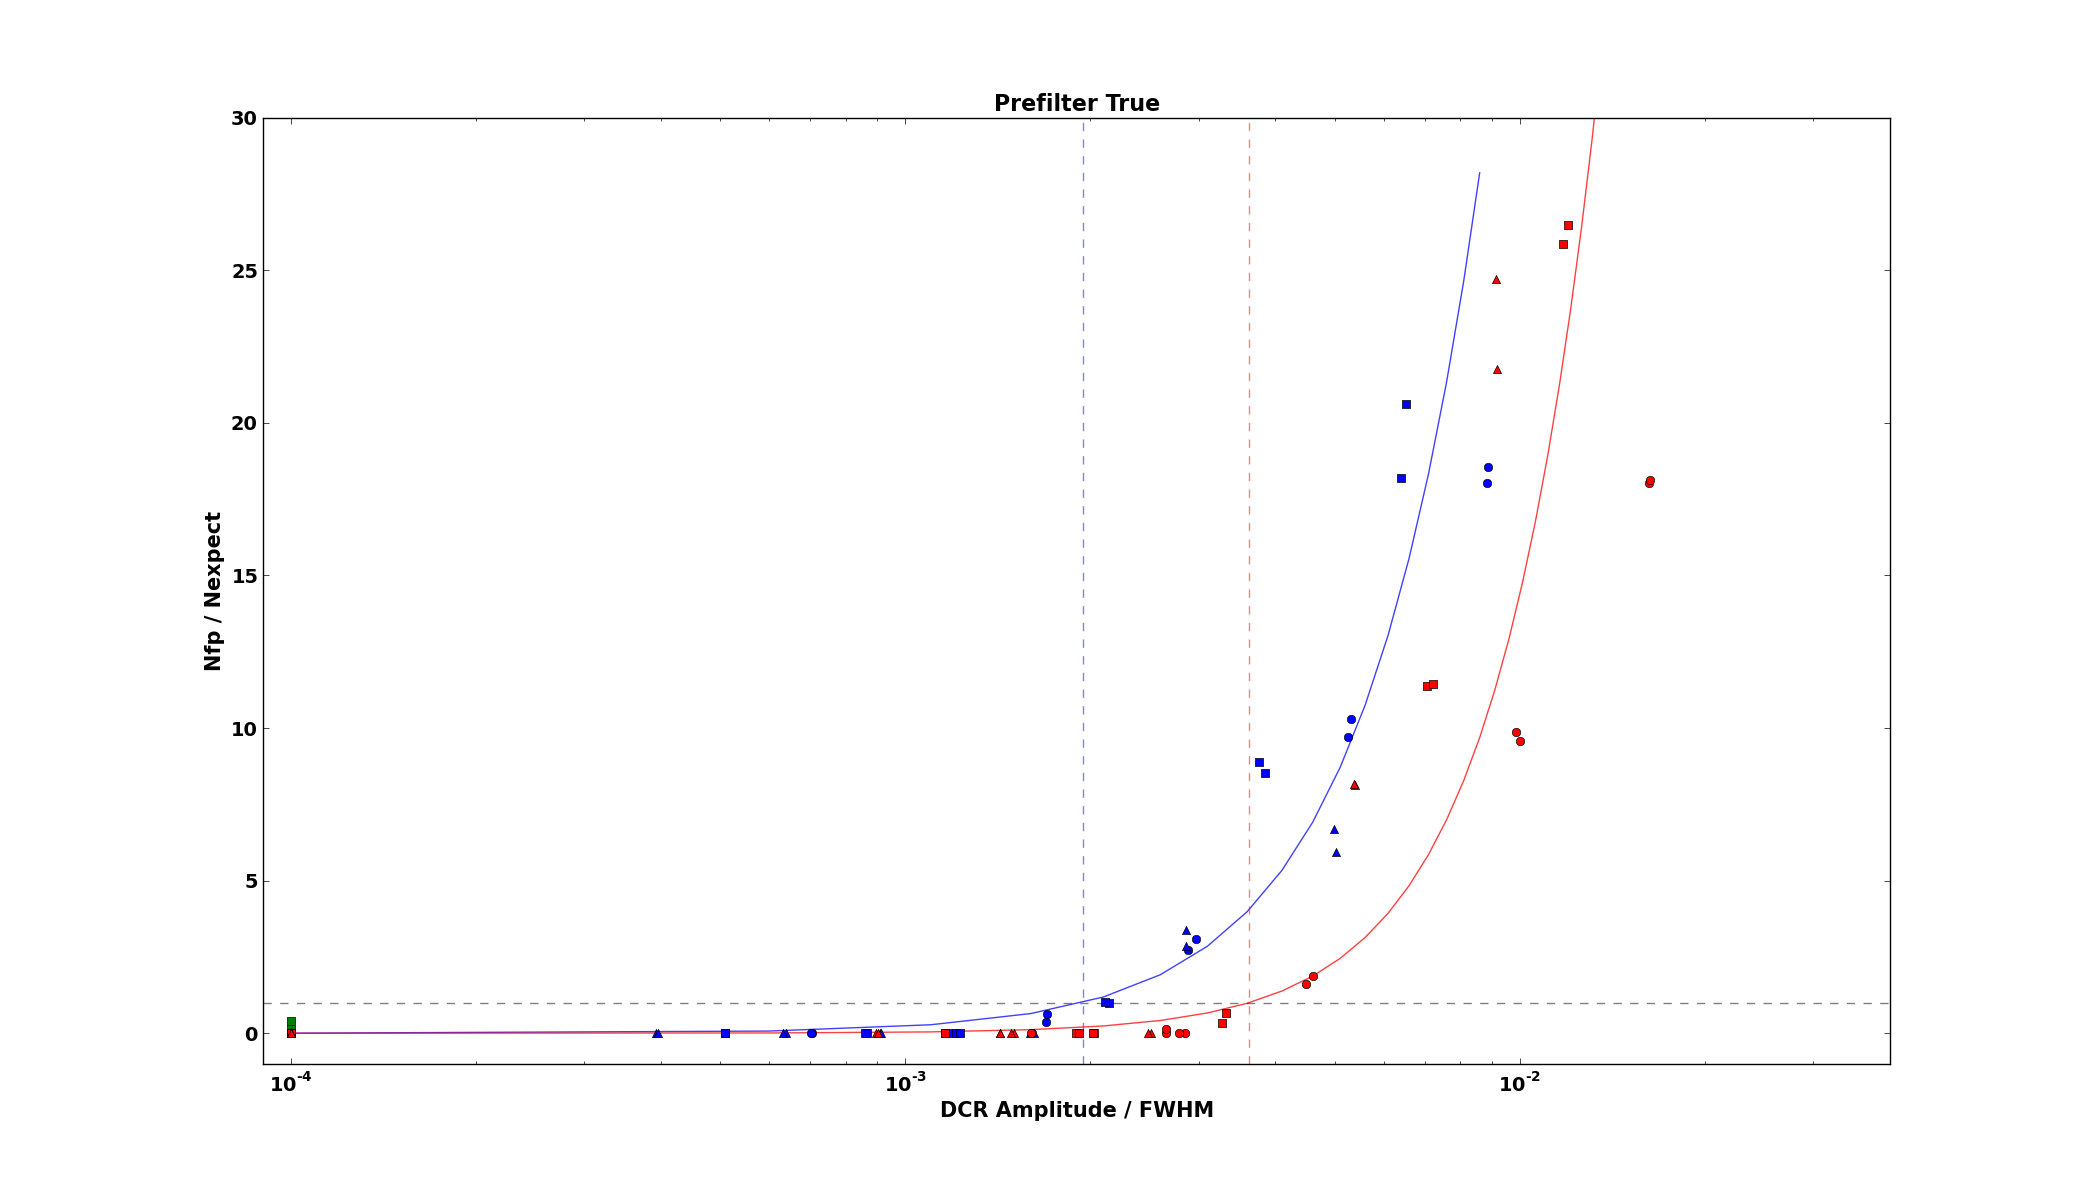
\includegraphics[width=0.65\textwidth]{regressTrue.png} }} \\
  \caption{{\bf DCR Impact on False Positives}: We plot the number of
    false positives that associate with {\tt A0V} stars as the blue
    points, and {\tt M2.0V} stars as the red points.  We normalize by
    the number expected due to fluctuations in the background, such
    that {\tt y=1} (horizontal black line) represents a doubling of
    false positives.  We plot this value as a function of the measured
    DCR offset determined via WCS residuals (Table~\ref{tab:dcramp}),
    normalized by the FWHM of the PSF.  We collapse information from
    all 3 passbands on this figure; the $i$--band data tend to have
    the smaller {\tt x}--values, and the $g$--band data larger values.
    We additionally include information from all 3 seeings by plotting
    seeing {\tt 1} data as {\it circles}, seeing {\tt 2} as {\it
      squares}, and seeing {\tt 3} as {\it triangles}.  We plot
    regressions of the form $log_{10}~y = a + b * log_{10}~x$ as solid
    lines, and the positions where these curves cross {\tt y=1} as
    vertical dashed lines.  This figure was created using the script
    {\tt python/fpRegressions.py}.}
  \label{fig:fpregress}
\end{figure}

\begin{figure}[!ht]
  \centering
  \subfloat[Prefiltering = False]{{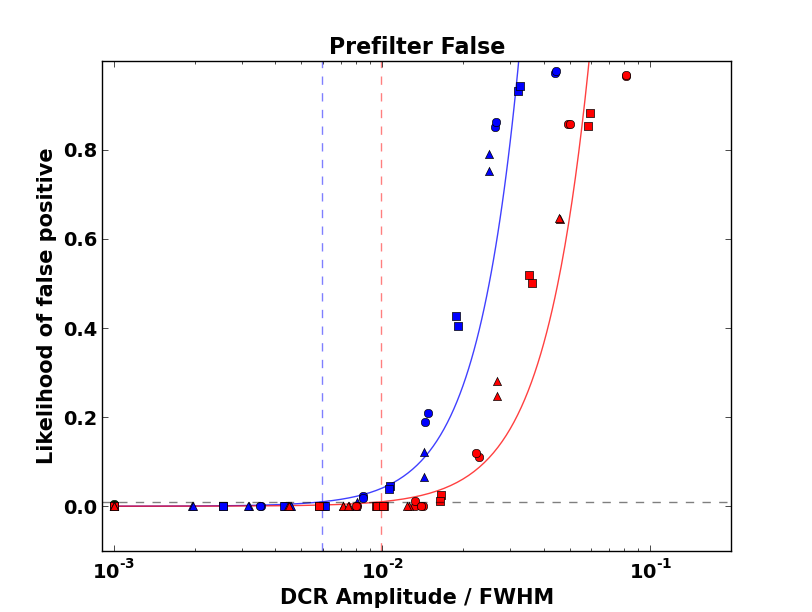
\includegraphics[width=0.65\textwidth]{regressFalse2.png} }} \\
  \subfloat[Prefiltering = True]{{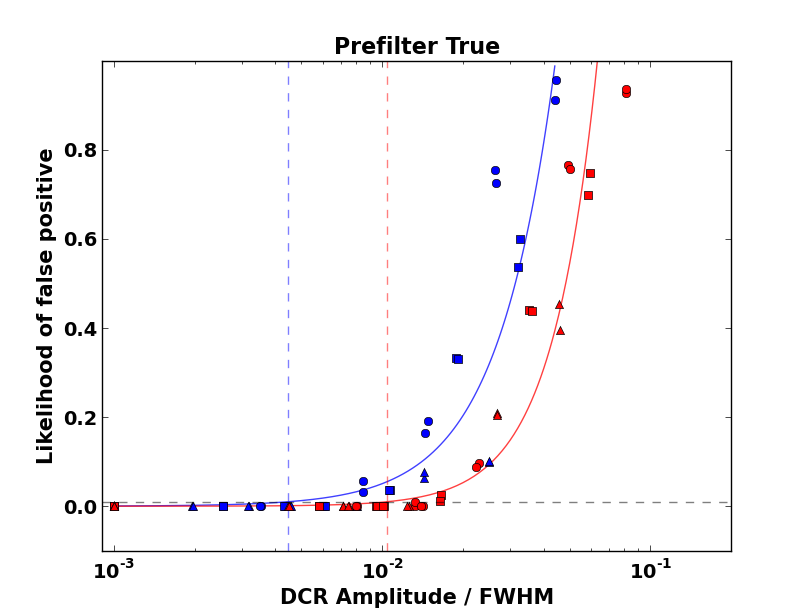
\includegraphics[width=0.65\textwidth]{regressTrue2.png} }} \\
  \caption{{\bf DCR Impact on False Positives}: Same as
    Figure~\ref{fig:fpregress}, but the {\tt y}--axis value represents
    the likelihood that an object of each spectral type will lead to a
    false positive.  This is appropriate for objects in the S/N range
    100-200, and for the SEDs used in this simulation.  Vertical lines
    are drawn where this curve crosses a 1\% likelihood.  This figure
    was created using the script {\tt python/fpRegressions2.py}.}
  \label{fig:fpregress2}
\end{figure}

\begin{figure}[!ht]
  \centering
  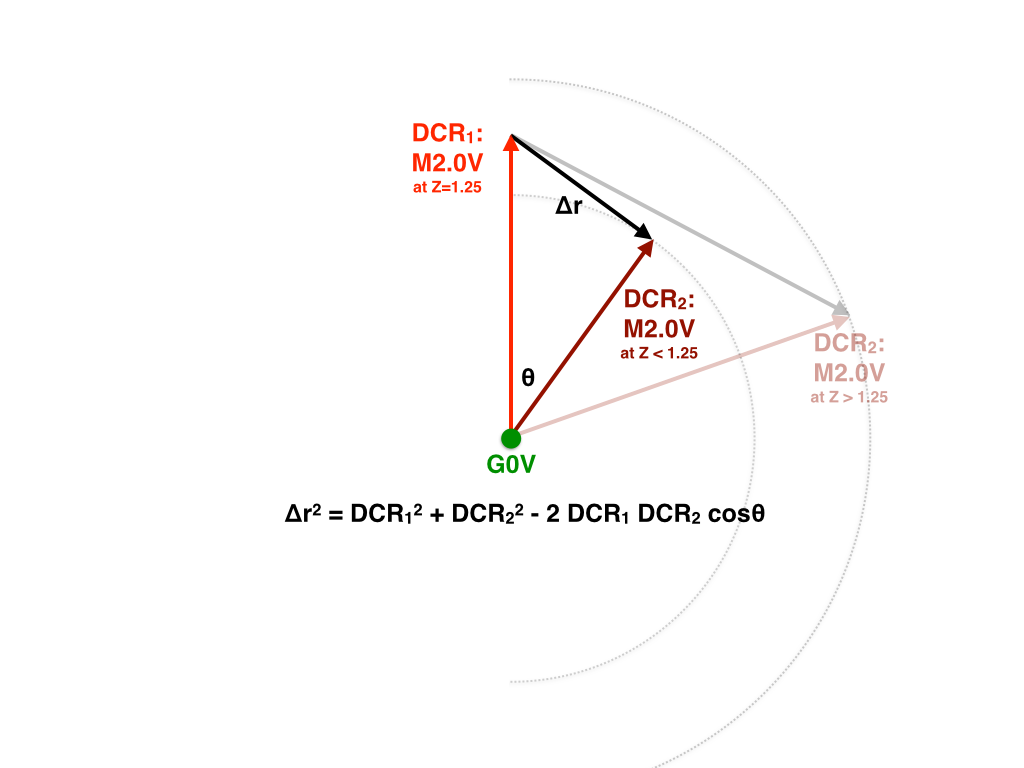
\includegraphics[width=1.0\textwidth]{DCR_001.png}
  \caption{{\bf Geometric Basis for Figure~\ref{fig:fpsummary}}: This
    figure provides the geometric basis for the study of astrometric
    offsets induced by DCR, as a function of difference in airmass and
    parallactic angle, for a single SED.  We use a reference DCR
    amplitude for the basis of this study, labeled here as {\tt DCR1}
    and representing the DCR of the {\tt M2.0V} star at 1.25 airmasses
    with respect to the {\tt G0V} star.  A second observation of this
    object is labeled {\tt DCR2}, and is observed at a different
    airmass (representing a different DCR amplitude, plotted along the
    {\tt y}--axis in Figure~\ref{fig:fpsummary}) and parallactic angle
    (denoted by theta, plotted along the {\tt x}--axis in
    Figure~\ref{fig:fpsummary}) than the reference observation.  The
    law of cosines is used to find the amplitude of the DCR offset
    $\Delta r$, which is used to color--code the panels in
    Figure~\ref{fig:fpsummary}.  The distance $\Delta r$ is
    effectively the distance from point {\tt DCR1} to the perimeter of
    the circle whose radius is {\tt DCR2}.}
  \label{fig:fpgeom}
\end{figure}

\begin{figure}[!ht]
  \centering
  \subfloat[$g$--band, 1.0 airmass template]{{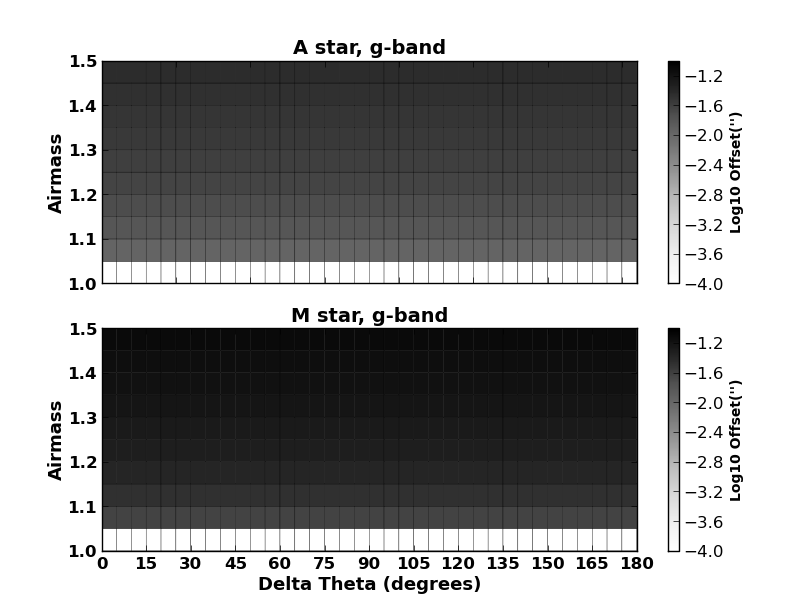
\includegraphics[width=0.29\textwidth]{dcrG1.png} }}
  \qquad
  \subfloat[$r$--band, 1.0 airmass template]{{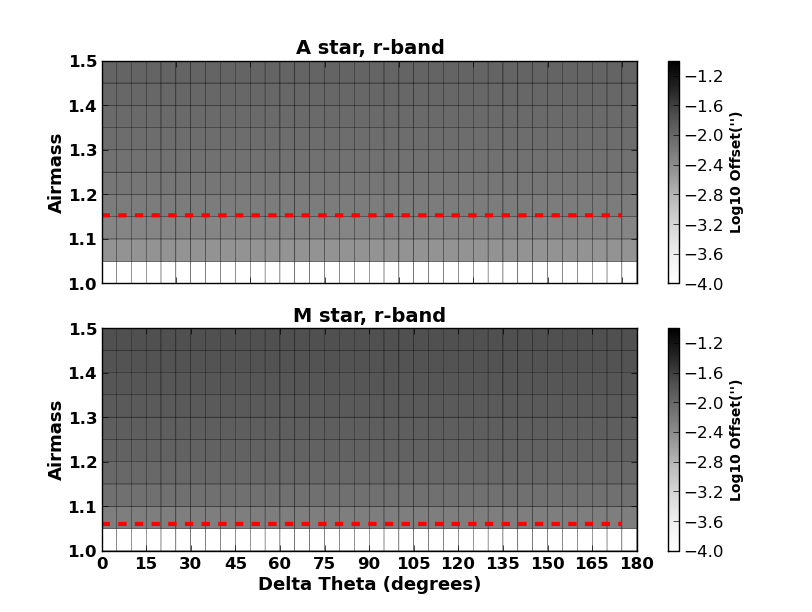
\includegraphics[width=0.29\textwidth]{dcrR1.png} }}
  \qquad
  \subfloat[$i$--band, 1.0 airmass template]{{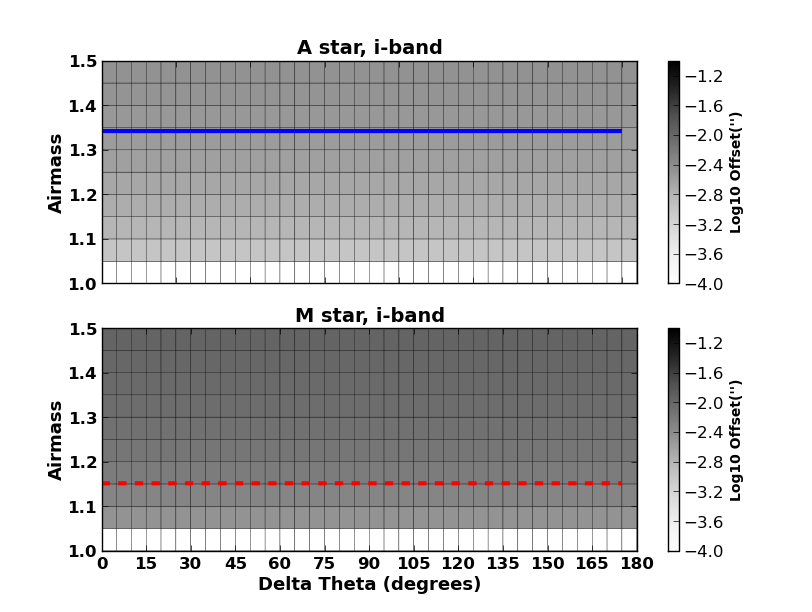
\includegraphics[width=0.29\textwidth]{dcrI1.png} }} \\
  \subfloat[$g$--band, 1.25 airmass template]{{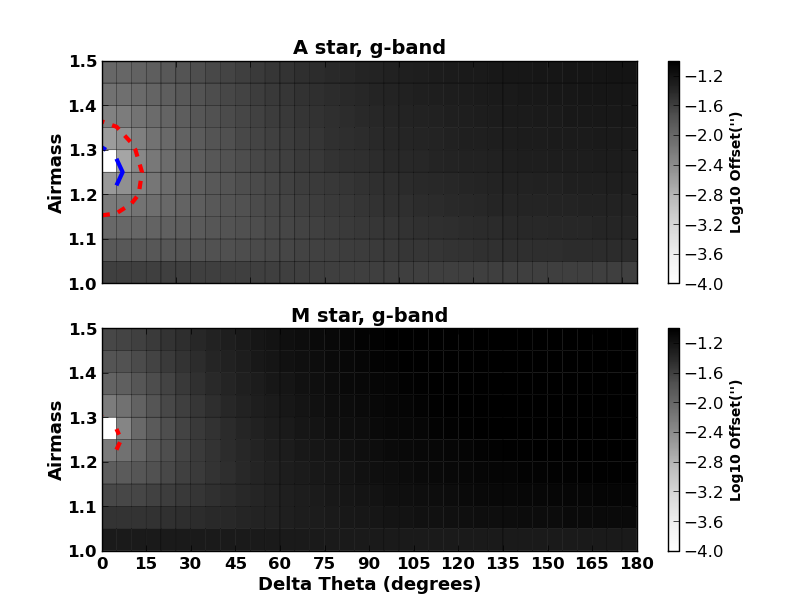
\includegraphics[width=0.29\textwidth]{dcrG125.png} }}
  \qquad
  \subfloat[$r$--band, 1.25 airmass template]{{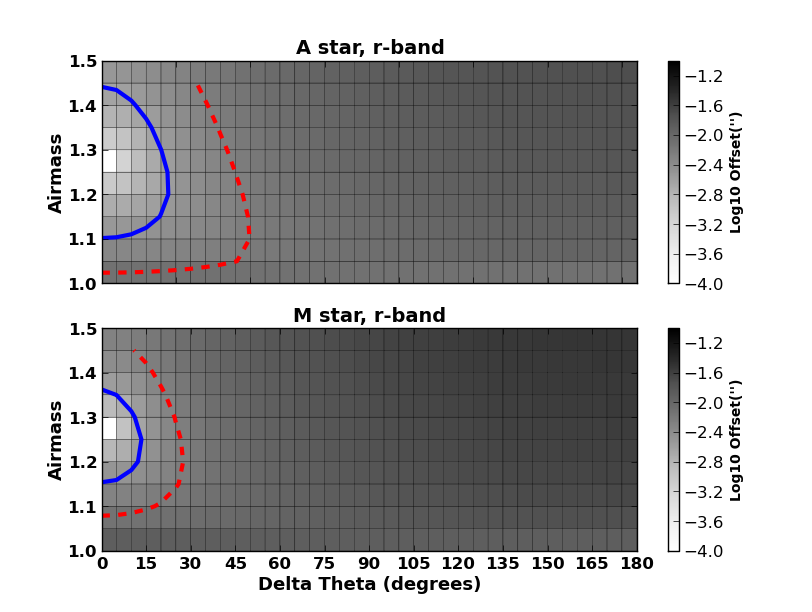
\includegraphics[width=0.29\textwidth]{dcrR125.png} }}
  \qquad
  \subfloat[$i$--band, 1.25 airmass template]{{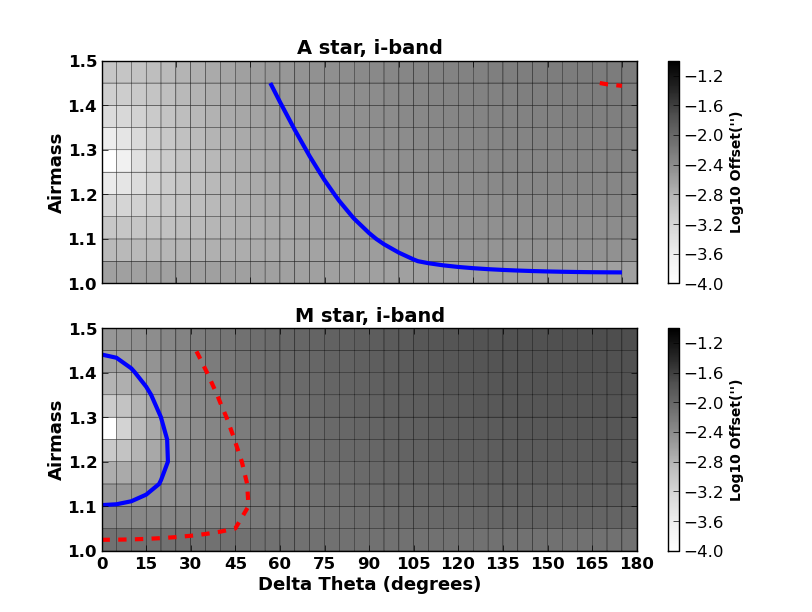
\includegraphics[width=0.29\textwidth]{dcrI125.png} }} \\
  \caption{{\bf DCR Offsets vs. Airmass and Orientation}: Each of
    these panels shows the amplitude of the relative DCR vector in
    arcseconds, calculated as a function of reference airmass (1.0 top
    row, 1.25 bottom row) and spectral type ({\tt A0V} star top
    subpanel in each, {\tt M2.0V} star bottom subpanel).  We calculate
    the DCR w.r.t. the {\tt G0V} star at each reference airmass, and
    subsequently calculate the DCR vector at other airmasses (encoded
    by the ordinate value) and parallactic angle orientations
    (abscissa).  The color of each pixel corresponds to the length of
    this differential DCR vector.  Contours of constant offsets are
    plotted at 3 mas in blue solid lines and 6 mas in red dashed
    lines, corresponding to the approximate DCR offsets yielding 1\%
    likelihood of a false positive (Figure~\ref{fig:fpregress2}) at a
    fiducial seeing of 0.6''.  We note that the top panels, with the
    reference observation at airmass 1.0, have no orientation
    dependence of this value because there is no DCR in the reference
    observation.
%
%    , but indicates that for the red objects, DCR will
%    start to dominate the false positive rate when differencing
%    against observations at airmasses 1.1--1.2.  The bottom panel,
%    with a reference observation at 1.25, demonstrates the combination
%    of airmass and orientation dependence on the DCR offsets.  As
%    demonstrated by the red star, observations at a similar airmass
%    but having differences in orientation of 35 degrees will yield
%    significant false positives.
%
    This figure was created using the script {\tt python/DCR3.py}.}
  \label{fig:fpsummary}
\end{figure}


\section{Thoughts on the DCR Issue}

We outline possible resolutions to the DCR issue.  Classes that need
to know about DCR include the {\tt WCS} class, for astrometric
modeling, and the {\tt Psf} class, for its contribution to the
color--dependent point spread function.  The consumers of this
information include the image coaddition and differencing tasks.  The
latter has a double dependency on DCR, since it uses coadded templates
whose generation themselves depends on an adequate treatment of DCR.
We expect to work towards this resolution in the upcoming Summer 2014
production (S14) cycle.

Modeling the expected effects of DCR should be relatively
straightforward, assuming the colors of most objects are known from
data release processing, the observation conditions are known exactly,
and the environmental conditions known approximately.  The majority of
objects whose instantaneous color is not known (moving objects, or
objects that change in brightness) will leave signatures in difference
images anyways, so not knowing their color should not create
additional ``false positives''.  It may however complicate the
measurement of these objects.  Places where this assumption breaks
down completely are for objects that are different in color but not
brightness, or for crowded fields where every pixel has its own color.

Compensating for the effects of DCR within an image requires not the
shifting of the image, but the shifting of every object {\it within}
the image along the vector to zenith.  This suggests a
color--dependence to the pixel resampling process, which might use both
the {\tt Wcs} and a putative {\tt Dcr} class to map the location of an
object to unrefracted coordinates (i.e. above the atmosphere).  This
would be extremely important if we wished to ``undo'' the effects of
DCR before coadding images taken at different airmasses and
parallactic angles.  We would also have to ``mimic'' DCR when mapping
coadded image subtraction templates to the science image conditions
(assuming that all pixel--level operations happen on the template
during image subtraction).  In these scenarios, neighboring pixels
must be treated as a bundle, to preserve the {\tt Psf}.  It is unclear
how to proceed when remapping e.g. a nearby galaxy, or a crowded
starfield in the Galactic plane.

The simplest solution is to reject objects (or pixels) of extreme
color from triggering alerts at high airmass.  A slightly more
complicated solution is to include the effects of DCR in measurement,
i.e. improve the dipole measurement code.  And the most complicated
option is the one described above, where DCR is compensated for at the
per--object pixel level, either during pixel remapping/resampling or
during {\tt Psf}/{\tt Psf}--matching kernel modeling.  We can take
some guidance from the analysis presented in Section~3.3 of
\citet{1999ApJ...521..602A}, who use a per--pixel color map to
compensate for DCR.  A necessary improvement over that technique is
the need to undertake this operation in a way that preserves the PSF.
A final option is to make this a consideration during the acquisition
of the data (e.g. observing a field within a narrow range of azimuth),
the feasibility of which may be tested via OpSim.

Other options are both solicited and welcome.

\section{Conclusions}

\begin{itemize}

\item We are able to qualitatively reproduce the results of W13,
  namely a false positive rate in difference images that is near the
  theoretical rate expected from fluctuations in the background.
  Quantitative differences reflect changes in both {\tt phoSim} and
  the DM stack since W13.  We find no filter--dependence to these
  results.

\item We find that the variance planes of the data products
  immediately following image subtraction are consistent with the
  empirical variance to 1\%.  This result holds for both the
  prefiltering and postfiltering analysis paths.

\item However, the convolution of an unfiltered difference image with
  its {\tt Psf} (i.e. the postfiltering process immediately preceding
  detection) results in an image whose variance plane provides a poor
  estimate of the true variance.  In the case of deconvolution of the
  template, this variance plane {\it overestimates} the true variance
  by 30--40\%, resulting in a lower rate of false positives but also
  shallower effective depth.  In the case of smoothing of the
  template, this variance is a 4--5\% {\it underestimate}, resulting
  in an enhanced rate of false positives.  This effect is only
  relevant for the postfiltering analysis path.

\item We find that differencing templates and images taken at the same
  airmass and parallactic angle -- regardless of airmass, parallactic
  angle, filter, or seeing -- generally produce the same high quality
  results.

\item We find that mismatches between parallactic angle, even for
  images taken at the same airmass, are sufficient to produce
  significantly enhanced rates of false positives in difference
  images, especially in the $g$--band and $r$--band.  Mismatches
  between both airmass and parallactic angle also yield enhanced false
  positive rates.  Accordingly, DCR is a substantial issue that needs
  to be addressed.

\item This enhanced false positive rate is more significant in the
  bluer passbands, but declines significantly by $i$--band.

\item The enhanced rate is also seeing dependent, in the sense that
  better seeing data yield more false positives than worse seeing
  data.

\item Two components in the false positive ``heat maps'' correspond to
  enhanced false positive rates in the no--refraction vs
  high--refraction data (\C\A\ and \C\E\ differences) and in the data
  with maximal mismatch between the DCR orientation vectors (\A\E\ and
  \E\A).

\item While the enhanced false positive rate is lower in the
  prefiltered difference images than in the postfiltered, it is not
  negligible.

\item Relative DCR offsets of 3--6 milliarcseconds allow a 1\% chance
  of a red/blue source yielding a dipole, at seeing of 0.6''.  This is
  relaxed to 5--9 mas in seeing of 0.88''.  This conclusion is
  restricted to the SEDs used in this study.  A comprehensive
  understanding of the number of stars that may yield DCR dipoles
  requires a realistic distribution of SEDs.

\item Templates obtained at zenith are applicable to a limited range
  of science data before DCR amplitudes reach 3--6 mas
  (Figure~\ref{fig:fpsummary}).

\item Templates imaged at airmass 1.25 are applicable to science data
  having differences in airmass of less than $0.05, 0.1, 0.15$ for
  $g,r,i$ or parallactic angle orientation differences of less than
  $5^{\circ}, 15^{\circ}, 25^{\circ}$.

\item Most/all image differences in the $u$--band and $g$--bands will
  be highly sensitive to this DCR effect.

\item The orientation of the DCR effect in the simulations is
  consistent with expectations.

\item We find that the amplitude of DCR shift in the red {\tt M2.0V}
  stars is under-realized by $\sim 10\%$ compared to expectations.
  {\tt A0V} stars are over-refracted by $\sim 4\%$ compared to
  expectations.

\item Dipole measurement measures lobe separations that are
  substantially larger than the effects of DCR.  This effect gets
  worse with seeing, indicating a potential need to improve the
  algorithm.

\item The treatment of DCR will likely be a complicated one, and at
  the extreme may require an object--dependent remapping during the
  image registration process.  Image subtraction is doubly dependent
  on this effect, as its template images need to first be coadded
  (which requires registration of input images {\it and} of the
  DCR--affected objects within the images) before being warped to the
  image coordinate system to be used for subtraction.

\item We further document the end--to--end process of creating and
  running simulated data in the Appendices below.

\end{itemize}

\bibliography{lsst,refs,books,refs_ads}

\appendix

\section{Test files}

The root directory for this analysis is located on the NCSA machines
at \\{\tt /nfs/lsst/home/becker/Winter2014}.  All files not included in
this {\tt git} repository may be found there, including the output
repositories needed by the majority of the analysis and plotting
scripts.  A complete guide to every step in this W14 process may be
found in the {\tt NOTES} file.

\section{Ticket Work}

\subsection{Ticket \#3128 \label{sec:3128}}

This ticket was opened to allow the user to select the sample of
``red'' and ``blue'' stars to be added to the control sample.  This
enabled after--the--fact diagnostics of the different populations of
objects.

\subsection{Ticket \#3143 \label{sec:3143}}

This ticket was opened to fix a bug in the settings of the
deconvolution kernel sizes.  A variable was unintentionally causing a
misconfiguration of the kernel basis in the $g$ and $r$--band
postfiltering seeing {\tt 1} data (which result in a deconvolution).
This resulted in a factor of 10--100 increase in the deconvolution
false positives, compared to the $i$--band.  This misconfiguration
results in the large numbers of false positives reported in
Section~\ref{sec:task1} below, and was fixed for the analysis of
Section~\ref{sec:task2}.  This indicates that deconvolution may be
undertaken with the proper kernel configuration, resulting in an
acceptable false positive rate, although the variance in the images
ends up being much higher (and the effective detection threshold much
lower) compared to the prefiltering route.

\subsection{Ticket \#3161 \label{sec:3161}}

This ticket was the most extensive implemented in this W14 work.
Previously, joint--Psf dipole measurement (simultaneously fitting for
a positive and negative--going {\tt Psf} with 6 model terms including
two x,y centroids and two fluxes) used a very coarse ``minimization''
routine.  This routine effectively took half pixel steps in the 4
centroid positions, and performed a linear fit for the two fluxes at
each step, returning the step that yielded the lowest $\chi^2$.
However, the dipole separations expected from DCR were in general far
smaller than the default step size, and thus the measurements were too
coarse for this task.  In addition, this process was slow and
inefficient, making measurement of more than $\sim 200$ dipoles in a
given image infeasible.

In Ticket \#3161 we implemented a fully non--linear joint {\tt Psf}
fit, using the {\tt Minuit} package.  This substantially sped up the
per--dipole measurement process by a factor of 20--30, from 1--2
measurements per second to 20--60 per second.  This speed--up analysis
was performed using script {\tt python/compareMeasurementTiming.py} in
this repository.  Dipole measurement is currently {\it not} the tall
pole in processing; resources should be spend on speeding up the
convolution and warping code to minimize the overall run time.


\section{Use of PhoSim}

I describe here the end-to-end process of generating instance catalogs
(or ``trim files'') for {\tt phoSim}, running these images to create
output {\tt eImages}, creating {\tt astrometry.net} index files for
astrometric calibration, and running these images through {\tt
  processEimage.py}.  This does {\it not} include the process of
generating instance catalogs from a master base catalog, or the
process of using calibration data to run the simulated images through
{\tt processCcd.py}, which does (amongst other operations) the
assembly of amp images into CCD images and instrument signature
removal.

The process is valid for {\tt phoSim} version 3.3.2.

\subsection{Setting up PhoSim}

To download, build, and setup {\tt phoSim}:

{\small
\begin{Verbatim}[frame=single]
wget https://dev.lsstcorp.org/cgit/LSST/sims/phosim.git/snapshot/phosim-3.3.2.tar.gz
tar -xzvf phosim-3.3.2.tar.gz
cd phosim-3.3.2
 -- or --
git clone http://dev.lsstcorp.org/git/LSST/sims/phosim
cd phosim

./configure
  n
  c
  $CFITSIO_DIR/lib/
  $CFITSIO_DIR/include/
  $FFTW_DIR/lib/
  $FFTW_DIR/include
make
mkdir ups
echo 'envPrepend (PATH, ${PRODUCT_DIR})' >> ups/phosim.table
echo 'envPrepend (PATH, ${PRODUCT_DIR}/bin)' >> ups/phosim.table
setup -k -r .
\end{Verbatim}
}

Note that you will have to declare the locations of {\tt cfitsio} and
{\tt fftw3} by hand, and must enter the full paths above (i.e. not the
string ``\$CFITSIO\_DIR/lib/'' but the path that it resolves to).  The
above assumes that you have a DM stack already, with {\tt cfitsio} and
{\tt fftw3} setup.

\subsection{Running {\tt phosim.py}}

To run {\tt phoSim}, you need the environment variable
CAT\_SHARE\_DATA declared, as this is where the package looks for its
SEDs.  Example locations are, at NCSA, {\tt
  /lsst/home/aconnolly/imsim/starSED/}.  You also need to create {\tt
  work/} and {\tt out/} directories for the script to use; these must
be made {\it before} the simulation is run.  A ``trim'' file or
instance catalog must be created, which contains a random seed and
observation information such as pointing, seeing, and the star catalog
itself.  These are included in this repository for all sims runs.  A
control file (named {\tt clean.params.beta} here) must also be
included, and turns off/on various effects in the sims, such as sky
backgrounds and tracking errors.  A call to the {\tt phoSim} package
then looks like:

{\small
\begin{Verbatim}[frame=single]
python $PHOSIM_DIR/phosim.py $PWD/2001000.trim -w $PWD/2001000.work -o $PWD/2001000.out
  -c $PWD/clean.params.beta
  -s "R22_S00|R22_S01|R22_S02|R22_S10|R22_S11|R22_S12|R22_S20|R22_S21|R22_S22" -p 16
\end{Verbatim}
}
where {\tt -w} defines the work directory (which must already exist),
{\tt -o} the output directory (which must already exist), {\tt -c} the
control file, {\tt -s} the sensors to simulate, and {\tt -p} the
number of cores to use.


Once the raw amplifier and {\tt eImages} are created, they need to be
renamed for consistency with the {\tt obs\_lsstSim} mapper.  The
repository script {\tt python/rename\_images.py} is used for this,
with an example command that moves the {\tt eImages} from the {\tt
  phoSim} output directory to a DM input directory called {\tt inputs8}:
{\small
\begin{Verbatim}[frame=single]
cd sims8/
foreach i (*.out)
 cd $i
 python ../../python/rename_images.py ../../inputs8 *E000.fits.gz
 cd ../
 end
\end{Verbatim}
}

Next, an input registry must be generated, and a mapper file created:

{\small
\begin{Verbatim}[frame=single]
cd inputs8/
python $OBS_LSSTSIM_DIR/bin/genInputRegistry.py .
echo "lsst.obs.lsstSim.lsstSimMapper.LsstSimMapper" >> _mapper
\end{Verbatim}
}

\subsection{Creating Astrometry Index Files}

A calibration file must be created for {\tt astrometry.net}, which is
used as the photometric and astrometric reference.  Typically this is
created from a base catalog, but since I am starting with instance
catalogs here, the process is somewhat different.  I use one of the
input trim files for this process as follows:

{\footnotesize
\begin{Verbatim}[frame=single]
mkdir astrometry_net_data8
python python/trim_to_ref.py sims8/2002000.trim > astrometry_net_data8/2002000.ref
cd astrometry_net_data8
setup -r /lsst/home/krughoff/lsst/lsst_devel/Linux64/astrometry.net-0.38/astrometry
text2fits.py 2002000.ref 2002000.fits
setenv P 1402120
build-index -i 2002000.fits -o index-${P}00.fits -I ${P}00 -P 0 -S r -n 100 -L 20 -E -j 0.4 -r 1
build-index -1 index-${P}00.fits -o index-${P}01.fits -I ${P}01 -P 1 -S r -L 20 -E -M -j 0.4
build-index -1 index-${P}00.fits -o index-${P}02.fits -I ${P}02 -P 2 -S r -L 20 -E -M -j 0.4
build-index -1 index-${P}00.fits -o index-${P}03.fits -I ${P}03 -P 3 -S r -L 20 -E -M -j 0.4
build-index -1 index-${P}00.fits -o index-${P}04.fits -I ${P}04 -P 4 -S r -L 20 -E -M -j 0.4
ls index-1402120* | awk '{printf("modhead %s+7 REFCAT '2002000'\n",$1)}' | sh
setup astrometry_net 0.30
cp -r /nfs/lsst/home/becker/Winter2014/astrometry_net_data/ups .
setup -k -r .
\end{Verbatim}
}

Note that the file {\tt andConfig.py} must be modified to use the
naming convention defined by environment variable {\tt P} above:

{\small
\begin{Verbatim}[frame=single]
cat astrometry_net_data8/andConfig.py
  root.starGalaxyColumn = "starnotgal"
  filters = ('u', 'g', 'r', 'i', 'z', 'y')
  root.magColumnMap = dict([(f,f) for f in filters])
  root.magErrorColumnMap = dict([(f, f + '_err') for f in filters])
  root.indexFiles = [
      'index-140212000.fits',
      'index-140212001.fits',
      'index-140212002.fits',
      'index-140212003.fits',
      'index-140212004.fits',
      ]
\end{Verbatim}
}

\subsection{Running processEimage.py}

Finally, the running of SFM via {\tt processEimage.py}:

{\small
\begin{Verbatim}[frame=single]
$OBS_LSSTSIM_DIR/bin/processEimage.py . --id visit=1000000^1001000^ .... -j 20
\end{Verbatim}
}
where {\tt -j 20} provides the number of concurrent threads.

\subsection{Running imageDifferenceWinter2013.py}

To difference all 3 seeing images from visit \A\ with a template from visit \C,
use the following command:
{\small
\begin{Verbatim}[frame=single]
$PIPE_TASKS_DIR/bin/imageDifferenceWinter2013.py inputs8 --id
  visit=3000001^3000002^3000003
  --output=/nfs/lsst/home/becker/Winter2014/outputs8CA_doPreConvolveFalse
  --configfile imageDifferenceConfigGstar.py --config diaSourceMatchRadius=2.0
  doAddCalexpBackground=False winter2013TemplateId=3002000  doPreConvolve=False
  subtract.kernel.active.singleKernelClipping=False
  subtract.kernel.active.kernelSumClipping=False
  subtract.kernel.active.spatialKernelClipping=False
  subtract.kernel.active.scaleByFwhm=True
  subtract.kernel.active.spatialKernelOrder=5 subtract.kernel.active.alardNGauss=3
  subtract.kernel.active.alardDegGauss="[5,2,2]"
  subtract.kernel.active.alardSigGauss="[1.0,1.0,1.0]"
  doSelectDcrCatalog=True --clobber-config -j 27
\end{Verbatim}
}

Important flags here are the W14 configuration file {\tt
  imageDifferenceConfigGstar.py}, the template visit via {\tt
  winter2013TemplateId}, and the prefiltering flag via {\tt
  doPreConvolve}.

\section{Generation of Instance Catalogs for W14 \label{appx:tasks}}

We outline the salient (and non--obvious) configuration parameters for
the W14 trim/instance catalogs below:
\begin{itemize}
  \item {\tt SIM\_MINSOURCE 1} : Only simulate the sensor if 1 or more
    stars land on it
  \item {\tt SIM\_VISTIME 300.0} : Total exposure time of the visit.
  \item {\tt SIM\_NSNAP 1} : Request one snap that accounts for all
    {\tt SIM\_VISTIME} seconds of the simulation.
\end{itemize}

In addition, the control file {\tt clean.params.beta} was designed to
turn off many confounding effects, such as tracking errors,
saturation, and blooming.  Specific trim file considerations for each
subtask are given below.

\subsection{Subtask 1}

We started with the trim files used in W13 processing, which consist
of a random star field populated by stars of SED {\tt
  km50\_5000.fits\_g20\_5140.gz}, and covering a range of magnitudes
$19 < r < 21$.  Observations were designed to be at a zenith distance
of $20.2^{\circ}$, with a boresight pointing of (Ra, Dec) =
($79.68926^{\circ}, -9.70229^{\circ}$).  Observations were simulated
in the $i$--band.  These trim files are stored in the {\tt sims3/}
directory in this repository.

\subsection{Subtask 2}

We chose spectrum {\tt km20\_6000.fits\_g30\_6020.gz} for our
reference {\tt G0V}-star, and replaced 80\% of the objects in the
original trim file with this SED.  We then selected the bluest object
contained in the base catalog, {\tt kp01\_9750.fits\_g45\_9830.gz},
for every tenth object starting at object \#0, and the most populous
red object in the catalog {\tt m2.0Full.dat.gz} for every tenth object
starting at object \#5.  These correspond to spectral types {\tt A0V}
and {\tt M2.0V}, respectively.

Because the magnitudes in the trim files represent a 500nm magnitude
(approximate $g$--band), color corrections to the requested magnitudes
of the objects were required to preserve the relative brightness
distribution of the as--simulated, multi--SED sources.  This was done
using their respective $i$--band magnitudes (i.e. a correction of
$-2.5~log_{10}~( f_{i;SED} / f_{i;GOV} )$).  Accordingly, the
brightness distributions in the $gr$--bands were not optimal (this was
fixed in subtask 3).  The colors of each spectral type were calculated
using {\tt python/colors.py}.  Script {\tt makeNewTrims.py} was used
to make these modifications to the {\tt sims3/} trim files, yielding
{\tt sims5/} trim files ($i$--band).  The only modifications made to
the input trim files to simulate images in the $gr$--bands were to
change the {\tt Opsim\_filter} field to indicate $gri$ = 123; these
are stored in the {\tt sims5gr/} directory.

\subsection{Subtask 3}

First, to have similar brightness distributions in all data, we make a
SED--dependent {\it and} passband--dependent magnitude correction to
the trim files used for this task.  These corrections are made in
script {\tt generateTrimFilesDcr.py}, which ran on the $i$--band trim
files from {\tt sims5}.

Second, the original observations do not pass through zenith on the
given night of simulated observations.  To design the observations to
pass through zenith at the LSST site, which is at southern latitude
$-29.67^{\circ}$, we first subtracted $19.96437^{\circ}$ from all
coordinates in the input trim files so that the field is centered at a
declination equal to the Southern latitude of the site.  This includes
both the per-object coordinates and the boresight pointing {\tt
  Unrefracted\_Dec} in the trim file header.

We simulated this star field throughout the night of MJD 51130 (the
night of the fiducial image simulations) to establish the times at
which it was at an altitude of 40 and 60 degrees (zenith distance of
50 and 30 degrees; airmass of 1.55 and 1.16), and when it was closest
to zenith.  We chose 5 specific times at which to simulate the images:
before meridian crossing at airmass 1.55; before meridian crossing at
airmass 1.16; closest to zenith; after meridian crossing at airmass
1.16; after meridian crossing at airmass 1.55).

Because the instance catalog inputs to {\tt phoSim} form an
overcomplete set (e.g. the user specifies Ra, Dec, altitude, azimuth,
and time of observation), it is possible to request a simulation
configuration that is not physically possible.  For this reason, we
used \\{\tt
  lsst.sims.catalogs.measures.example\_utils.makeObsParamsRaDecSky}
subroutine \\{\tt makeObsParamsRaDecSky} to generate a self--consistent
set of observation parameters given the Ra and Dec of the field, and
the times of observation established above.

In addition, this script synchronized the values of {\tt
  Opsim\_rotskypos} and {\tt Opsim\_rottelpos}.  {\tt Rotskypos} sets
the orientation of Ra and Dec of the catalog, effectively a rotation
of the Pole away from the Zenith.  When {\tt rotskypos=0} the Ra
direction is ``up'' in the image, along the y--axis.  This value was
kept the same for all images, so that the star field was always
rendered in approximately the same orientation.  {\tt Rottelpos} is
defined as ({\tt rotskypos}-180+parallactic angle), such that the
angle of DCR should be along this axis.  This will also be the angle
of increasing Altitude in the Az,Alt coordinate system.  This value is
observation dependent, and was determined using {\tt
  makeObsParamsRaDecSky}.  Trim files for this run are found in the
{\tt sims8/} directory of this repository.

\section{Refraction and DCR Overlays}

We provide here additional figures here that demonstrate the amplitude
of the refraction, of the differential refraction, and the airmass and
passband--dependent quality of the difference images.

\begin{figure}[!ht]
  \centering
  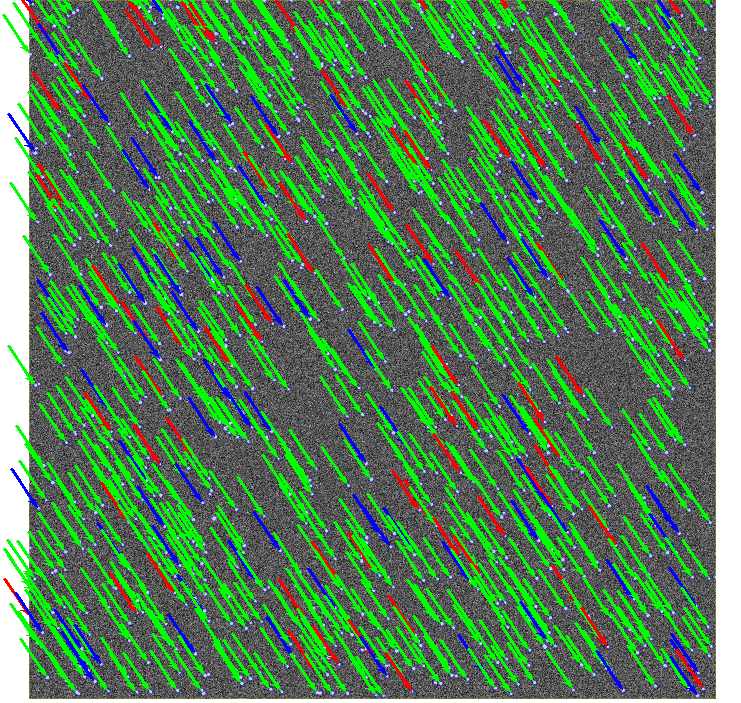
\includegraphics[width=0.5\textwidth]{outputs8bCA_g_doPreConvolveFalse_refract_crop.png}
  \caption{{\bf Refraction}: This figure depicts the amplitude and
    orientation of the refraction vector in the visit \A, {\tt
      raft=2,2 sensor=1,1 filter=g}, seeing value {\tt 2} data.  The
    vectors point from the unrefracted locations to the realized
    locations in the image.  The SEDs of the sources are indicated
    with colors {\tt blue}, {\tt green} and {\tt red} for {\tt A0V},
    {\tt G0V}, and {\tt M2.0V} respectively.  This figure was created
    using the script {\tt python/compareDcrFromSims.py}.}
  \label{fig:refractim}
\end{figure}

\begin{figure}[!ht]
  \centering
  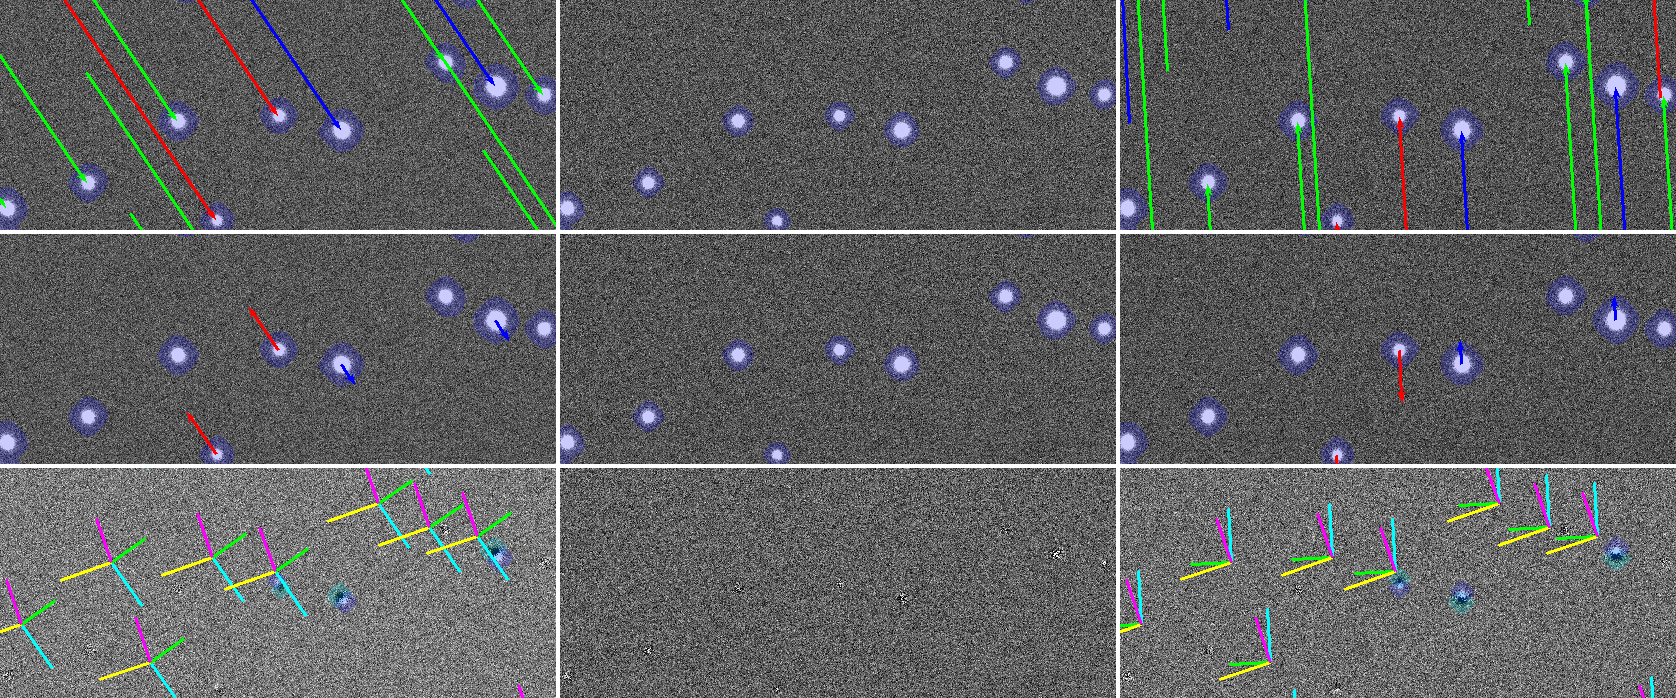
\includegraphics[width=1.0\textwidth]{outputs8b_g_doPreConvolveFalse_dcr_crop.png}
  \caption{{\bf Differential Chromatic Refraction and Difference Image
      Quality, $g$--band}: This set of panels demonstrates the amount
    of refraction (top row), differential refraction with respect to
    the {\tt G0V} star (middle row), and the quality of the difference
    image (bottom row) for three sets of image differences.  The first
    column uses science visit \A, the middle \C, and the third \E.  In
    all cases the template used was taken at zenith, i.e. visit \C.
    The top rows effectively present the same information as
    Figure~\ref{fig:refractim}, but zoomed in on a particular cluster
    of stars.  The second row subtracts off the green vector from all
    vectors.  The residual refraction of the blue,red vectors
    represents differential chromatic refraction.  These residual
    lengths have been multiplied by a factor of 100 for readability.
    Note that the blue vectors point along the vector to zenith,
    indicating the blue stars appear higher in the sky than their
    green counterparts, compared to an unrefracted observation.  The
    red stars are not refracted as much and thus will appear lower in
    the sky.  On the bottom row, we show the realized difference image
    quality.  Note that the blue stars have positive lobes pointing
    along the direction to zenith, meaning the stars are ``higher'' in
    the sky w.r.t. the green stars when compared to the zenith
    template, while the dipoles of the red stars have the opposite
    polarity.  For completeness, the Wcs--derived orientation of the
    Ra,Dec and Az,Alt coordinate axes are shown in the difference
    image (Ra,Dec,Az,Alt are magenta,yellow,green,cyan); see
    Figure~\ref{fig:wcsdcr} for more detail.  This figure was created
    using the script {\tt python/compareDcrFromSims.py}.}
  \label{fig:dcrimg}
\end{figure}

\begin{figure}[!ht]
  \centering
  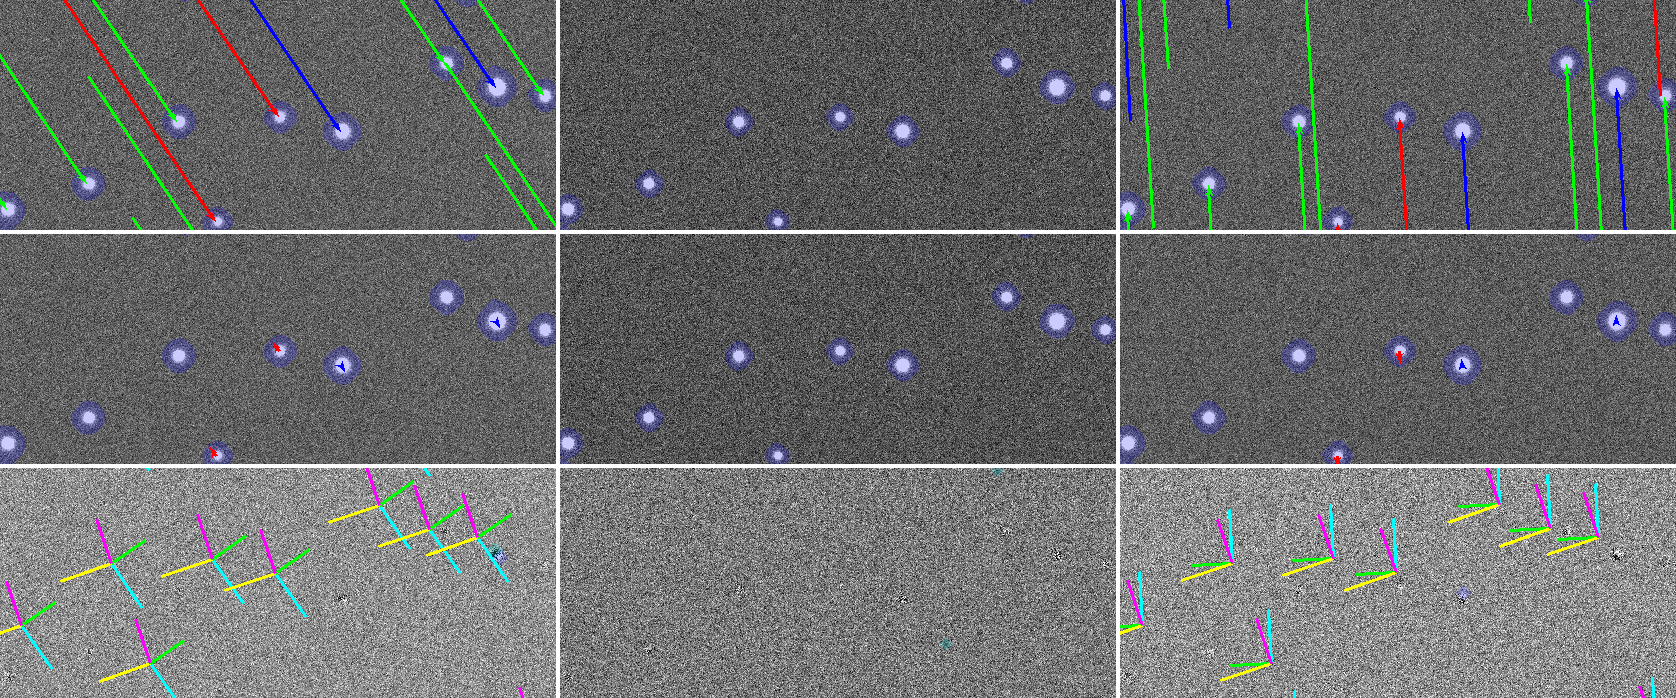
\includegraphics[width=1.0\textwidth]{outputs8b_r_doPreConvolveFalse_dcr_crop.png}
  \caption{{\bf Differential Chromatic Refraction and Difference Image
      Quality, $r$--band}: Same as Figure~\ref{fig:dcrimg}, but for
    $r$--band data.  This figure was created using the script {\tt
      python/compareDcrFromSims.py}.}
  \label{fig:dcrimr}
\end{figure}

\begin{figure}[!ht]
  \centering
  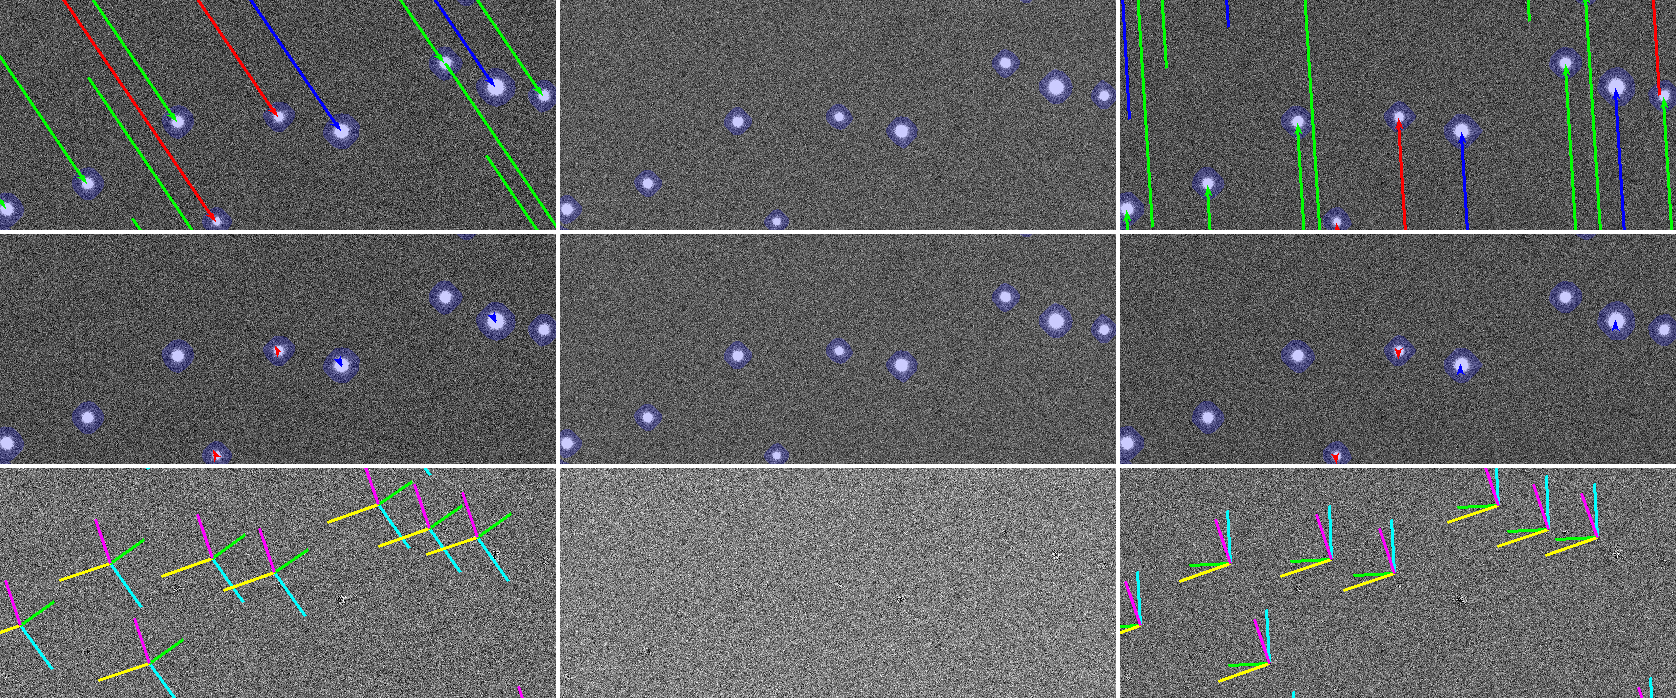
\includegraphics[width=1.0\textwidth]{outputs8b_i_doPreConvolveFalse_dcr_crop.png}
  \caption{{\bf Differential Chromatic Refraction and Difference Image
      Quality, $i$--band}: Same as Figure~\ref{fig:dcrimg}, but for
    $i$--band data.  This figure was created using the script {\tt
      python/compareDcrFromSims.py}.}
  \label{fig:dcrimi}
\end{figure}

\begin{figure}[!ht]
  \centering
  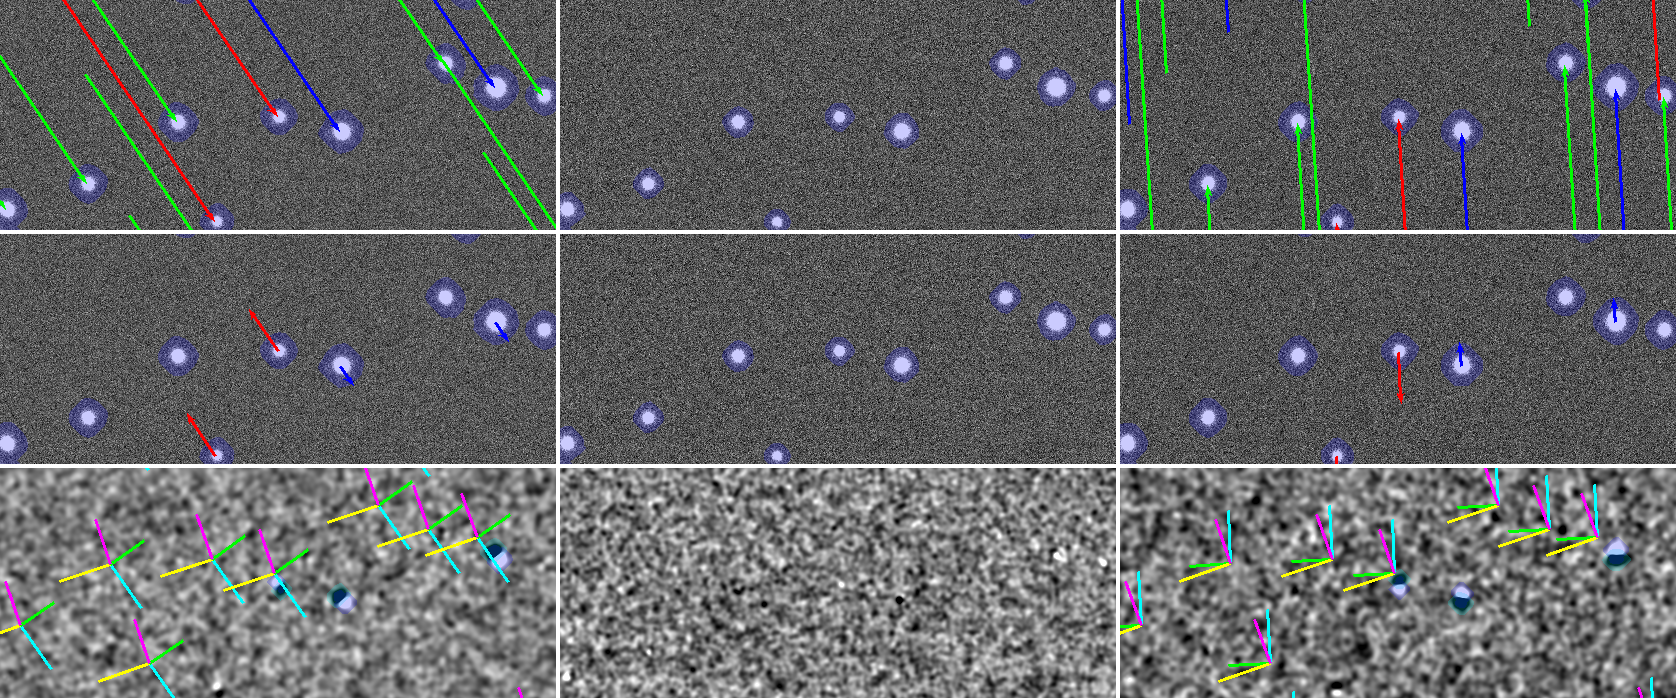
\includegraphics[width=1.0\textwidth]{outputs8b_g_doPreConvolveTrue_dcr_crop.png}
  \caption{{\bf Differential Chromatic Refraction and Difference Image
      Quality, Prefiltering}: Same as Figure~\ref{fig:dcrimg}, but
    using prefiltering of the science image with its Psf.  This figure
    was created using the script {\tt python/compareDcrFromSims.py}.}
  \label{fig:dcrimgpre}
\end{figure}


\end{document}
